% Anonymous regional-final technical document.  It reuses the local zjuthesis
% typography and bibliography stack, but intentionally omits thesis cover pages.
\documentclass[
    TwoSide=false,
    Degree=graduate,
    GradLevel=master,
    Type=thesis,
    Title={光电混合运动想象脑机接口技术文档}
]{zjuthesis}

\usepackage{amsmath}
\usepackage{array}
\usepackage{longtable}
\usepackage{url}
\graphicspath{{figure/}}
\addbibresource{competition_report.bib}
\hypersetup{colorlinks=true,linkcolor=black,citecolor=black,urlcolor=black}
\newcolumntype{L}[1]{>{\raggedright\arraybackslash}p{#1}}
\newcolumntype{Y}{>{\raggedright\arraybackslash}X}
\renewcommand{\TitleTypeName}{第十届集创赛复赛技术文档}
\newcommand{\projectname}{光电混合运动想象脑机接口}
\newcommand{\photonic}{\textbf{光计算映射}}
\newcommand{\digital}{\textbf{数字端处理}}

\begin{document}
\begin{titlepage}
  \thispagestyle{empty}
  \centering
  \vspace*{2.0cm}
  {\heiti\zihao{1} \projectname\par}
  \vspace{0.45cm}
  {\heiti\zihao{3} 基于曦智科技光子计算平台的 AI 应用创新与探索\par}
  \vspace{1.3cm}
  \rule{0.82\textwidth}{0.8pt}\par
  \vspace{0.5cm}
  {\zihao{3}\heiti 复赛技术文档\par}
  \vspace{0.35cm}
  {\zihao{4}版本 1.0 \quad 2026 年 7 月\par}
  \vspace{0.5cm}
  \rule{0.82\textwidth}{0.8pt}\par
  \vfill
  \vspace*{1.5cm}
\end{titlepage}

\prevstyle
\chapter*{作品核心内容快速预览}
\addcontentsline{toc}{chapter}{作品核心内容快速预览}
\noindent\textbf{作品目标。} 本项目面向运动想象脑机接口（MI-BCI）。这类系统常见的问题是：不同使用者的脑电差异较大，新使用者需要较长的校准时间，便携设备的计算资源也有限。为此，我们搭建了一条完整流程：从 EEG 中提取特征，再用小型网络和经验库选择合适的候选模型，最后用光计算仿真完成候选评分。系统输出左手、右手、脚三类运动想象指令；当结果不可靠时，输出 ``拒识''，不强行给出指令。

\vspace{0.35cm}
\noindent\textbf{核心流程。}
\begin{center}
\fbox{\parbox{0.90\linewidth}{\centering
\resizebox{0.96\linewidth}{!}{EEG $\rightarrow$ FBCSP $\rightarrow$ small MLP embedding $\rightarrow$ experience library $\rightarrow$ photonic scan $\rightarrow$ reject/command}}}
\end{center}

\vspace{0.15cm}
\noindent 系统先从 EEG 中提取 FBCSP 时频--空间特征，再由小型 MLP 将其编码为紧凑嵌入；经验库利用少量校准窗口选择并加权候选线性头，光计算扫描候选得到融合概率，最后根据置信度和间隔阈值输出运动想象指令或拒识结果。

\vspace{0.35cm}
\noindent\textbf{核心创新。}
\begin{enumerate}[leftmargin=2.2em,itemsep=0.15em]
  \item 用 FBCSP 从脑电中提取有物理含义的特征，再压缩成 32 维向量。系统只需少量校准窗口，就能在历史经验库中找相近的候选模型，不必从头训练。
  \item 每个窗口不只使用一个固定分类器，而是扫描 top-$K$ 个候选线性头，再按权重融合结果。这里的矩阵乘适合按 $2\times8$ tile 切块，是光计算仿真的主要部分。
  \item 同时检查信号质量、分类置信度和候选之间是否一致。只要其中一项不可靠，系统就拒识；只有稳定会话才会写入经验库。
\end{enumerate}

\vspace{0.2cm}
\noindent\textbf{当前证据。} 在 BCICIV\_1\_asc 回放实验中，42 个校准窗口仅用于经验库查询和候选加权，其余 518 个窗口用于在线评估；当前主线的指令准确率为 $70.46\%$，平衡准确率为 $73.24\%$，接受窗口准确率为 $72.42\%$，拒识率为 $2.70\%$。在 BNCI2014\_004 的 9 位被试实验中，主线平均准确率为 $74.92\%$，拒识率为 $1.62\%$。代码、测试、指标、单窗口推理入口和图表均已保存；候选头路径已完成量化、$2\times8$ tile 调度、光计算模拟器输出读回和计算量统计。Cyton 在线采集与上位机仍在完善，尚未完成真实 EEG 采集--推理--反馈闭环；当前结论来自公开数据集回放和光计算模拟器，不能表述为真实光芯片实测。

\vspace{0.4cm}
\noindent\textbf{复赛交付对应关系。}
\begin{center}\small
\begin{tabularx}{0.96\linewidth}{|L{0.20\linewidth}|X|}\hline
材料 & 支撑内容 \\ \hline
技术文档 & 方案、公式、实验协议、结果、计算量与实现边界 \\ \hline
源码与测试 & 三条实验线、backend、单窗口推理和回归验证 \\ \hline
metrics/figures & JSON/NPZ 原始指标、可追溯图表与计算账本 \\ \hline
PPT/视频 & 系统流程、公开数据回放、候选扫描和拒识展示 \\ \hline
\end{tabularx}
\end{center}

\clearpage
\tableofcontents
\clearpage
\listoffigures
\clearpage
\listoftables

\bodystyle
\fancypagestyle{competition}{\fancyhead[L]{\zihao{-5}\songti 第十届集创赛复赛技术文档}\fancyhead[R]{\zihao{-5}\songti \leftmark}\fancyfoot[C]{\zihao{-5}\songti \thepage}\renewcommand{\headrulewidth}{0.6pt}}
\pagestyle{competition}
\assignpagestyle{\chapter}{competition}

\chapter{问题定义与方案概述}
\section{运动想象 EEG-BCI 任务与信号挑战}
运动想象（motor imagery，MI）指使用者只在脑中想象肢体动作而不真正运动。系统接收一段多通道 EEG 决策窗口 $X\in\mathbb{R}^{C\times T}$，需要识别其中的左手、右手或脚运动想象意图，并把分类结果转换为控制命令；若信号质量或判别置信度不足，则输出拒识，避免把不可靠结果直接发送给外部设备。图~\ref{fig:mi-task}给出这一任务边界。
\begin{figure}[H]\centering
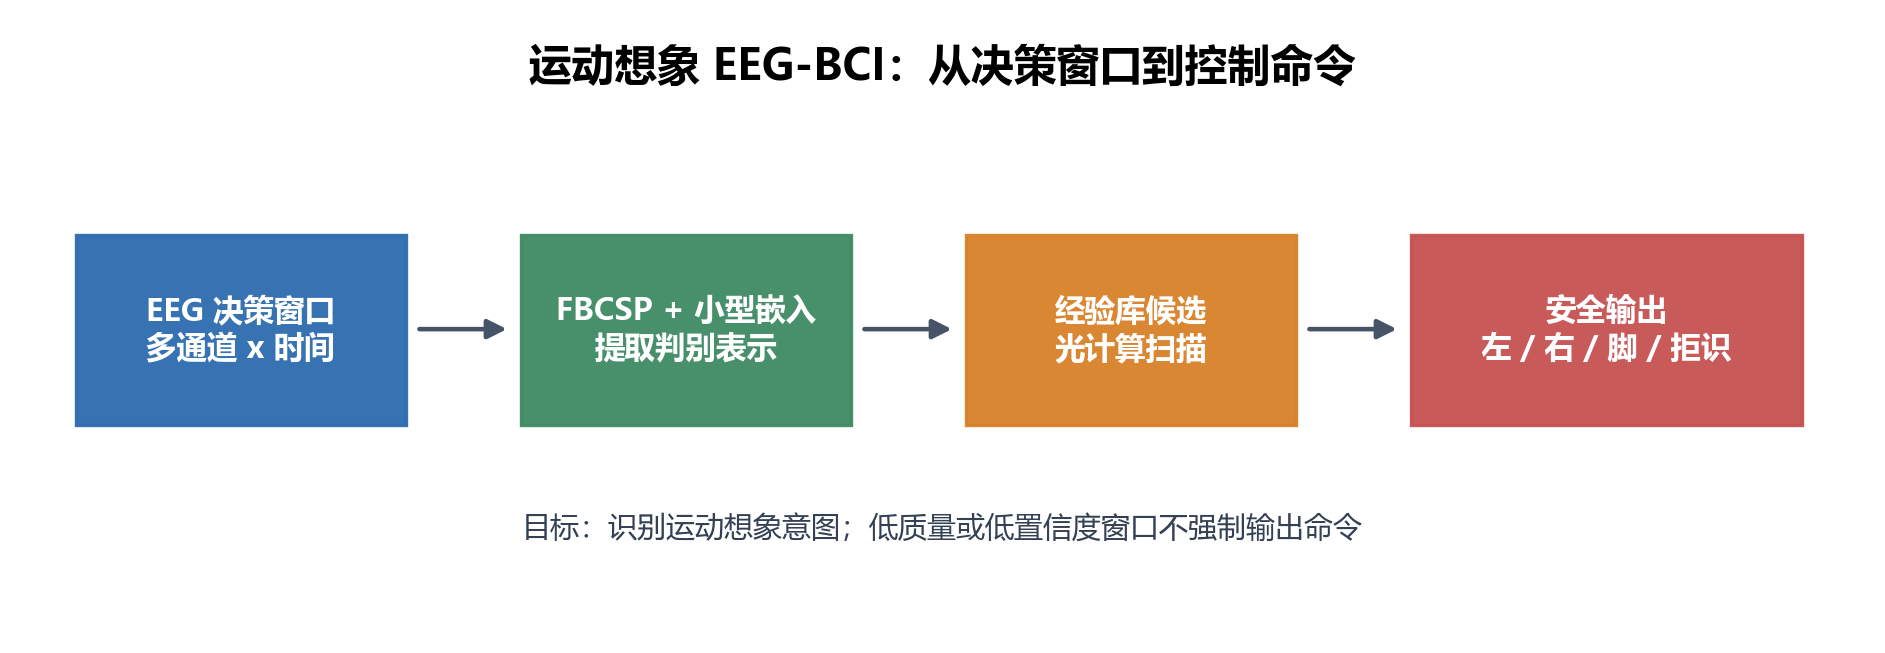
\includegraphics[width=0.92\linewidth]{competition/mi_bci_task_overview.png}
\caption{MI-BCI 任务示意：系统从一个多通道 EEG 决策窗口推理运动想象意图，并输出控制命令或拒识。该图为系统任务说明，不是实验结果。}\label{fig:mi-task}
\end{figure}

EEG 是头皮电极记录到的微弱电活动，具有低信噪比、小样本、非平稳和易受伪迹影响等特点。电极接触变化、眨眼、肌肉活动、工频干扰以及被试状态变化，都可能使同一任务在不同时段呈现不同分布。竞赛数据和实际校准数据通常又远少于图像、文本等任务的数据规模，因此模型不能只追求层数和参数量；它还需要可解释、对小样本稳定，并能明确处理坏窗口和会话漂移。

\section{脑电基础、电极位置与 MI 节律}
国际 10--20 系统用相对头部解剖位置规定电极名称：字母表示脑区，奇数和偶数通常分别表示左、右侧，$z$ 表示中线。C3、Cz、C4 位于中央区，靠近感觉运动皮层；左右手运动想象常在对侧中央区出现更明显的节律变化，Cz 及 FC、CP 邻近通道则补充中线与中央区前后方向的信息。本项目在线原型以 C3、C4、Cz、FC3、FC4、CP3、CP4、CPz 为目标 8 通道，公开数据实验则遵循数据集实际通道定义。

\begin{figure}[H]\centering
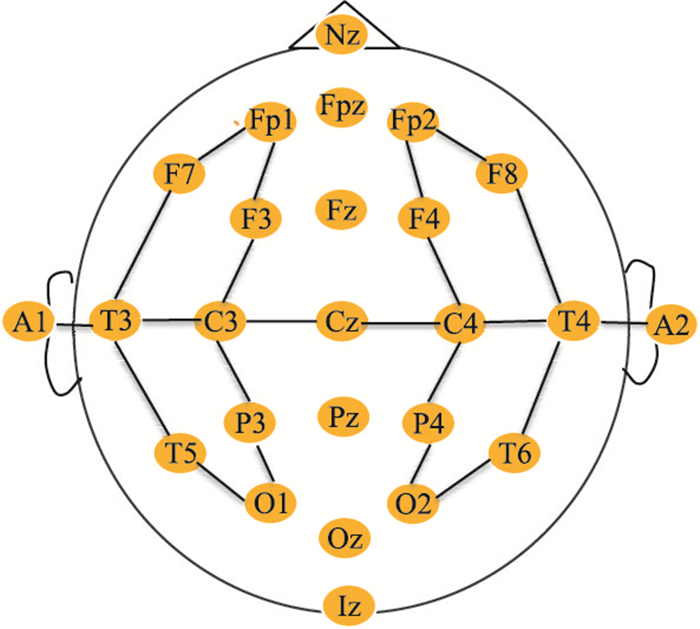
\includegraphics[width=0.56\linewidth]{competition/eeg_1020_electrodes.jpg}
\caption{国际 10--20 电极位置示意。项目重点使用中央区 C3、Cz、C4 及其前后邻近通道；图为电极命名和空间关系说明。}\label{fig:eeg-electrodes}
\end{figure}

使用者开始运动想象后，对侧感觉运动区的 mu 节律（约 8--12 Hz）和 beta 节律（约 13--30 Hz）功率常会降低，这称为事件相关去同步化（ERD）；想象结束或回到静息后，局部功率可能回升，称为事件相关同步化（ERS）。这些现象解释了系统为什么重点关注约 8--30 Hz 的运动相关节律，并同时观察多个频带和空间通道。图~\ref{fig:eeg-erd}用合成信号说明 cue 后的节律功率变化，仅是概念图，不是本项目实测数据。
\begin{figure}[H]\centering
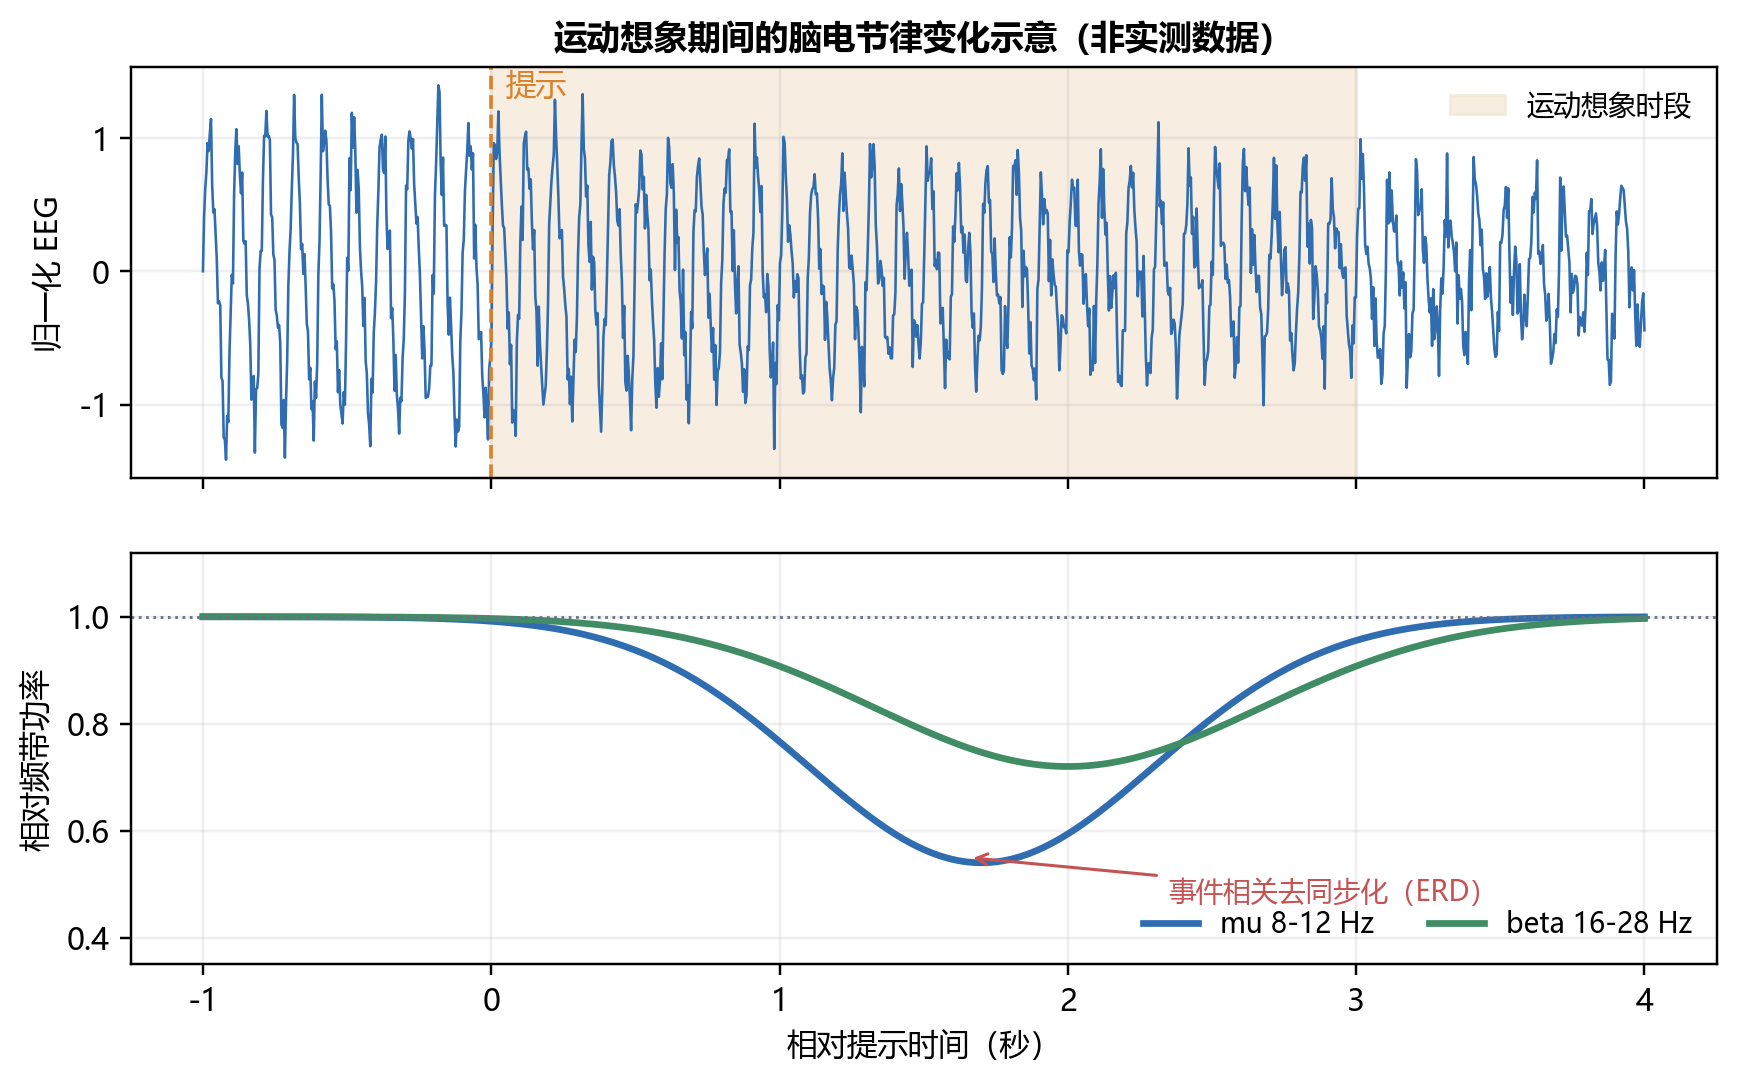
\includegraphics[width=0.93\linewidth]{competition/eeg_mi_signal_concepts.png}
\caption{运动想象 EEG 节律变化的概念可视化。上图为含噪节律波形，下图示意 cue 后 mu/beta 相对功率下降（ERD）；仅用于解释信号现象。}\label{fig:eeg-erd}
\end{figure}

\section{个体差异与会话特化动机}
运动想象 EEG 的跨被试差异尤其明显。不同人的有效节律响应可能落在不同子频带，C3/Cz/C4 及邻近通道上的空间激活模式也不相同；即使执行相同提示，被试采用的视觉想象、动觉想象和注意策略也会改变脑电表现。同一被试在不同日期还会受到电极位置、疲劳和学习效应影响。因此，一个对所有被试固定的泛化分类器未必能稳定覆盖新会话。

本项目主线采用“共享主干 + 少量校准后的个体/会话特化”。经验库保存由历史 EEG/MI 会话训练得到的特征中心、候选线性头和质量统计；新会话用少量校准窗口检索、评价并加权候选，而不是把经验库当作普通数据缓存，也不是从头训练大型网络。图~\ref{fig:specialization-logic}展示了个体差异、经验库特化和候选扫描之间的因果关系。
\begin{figure}[H]\centering
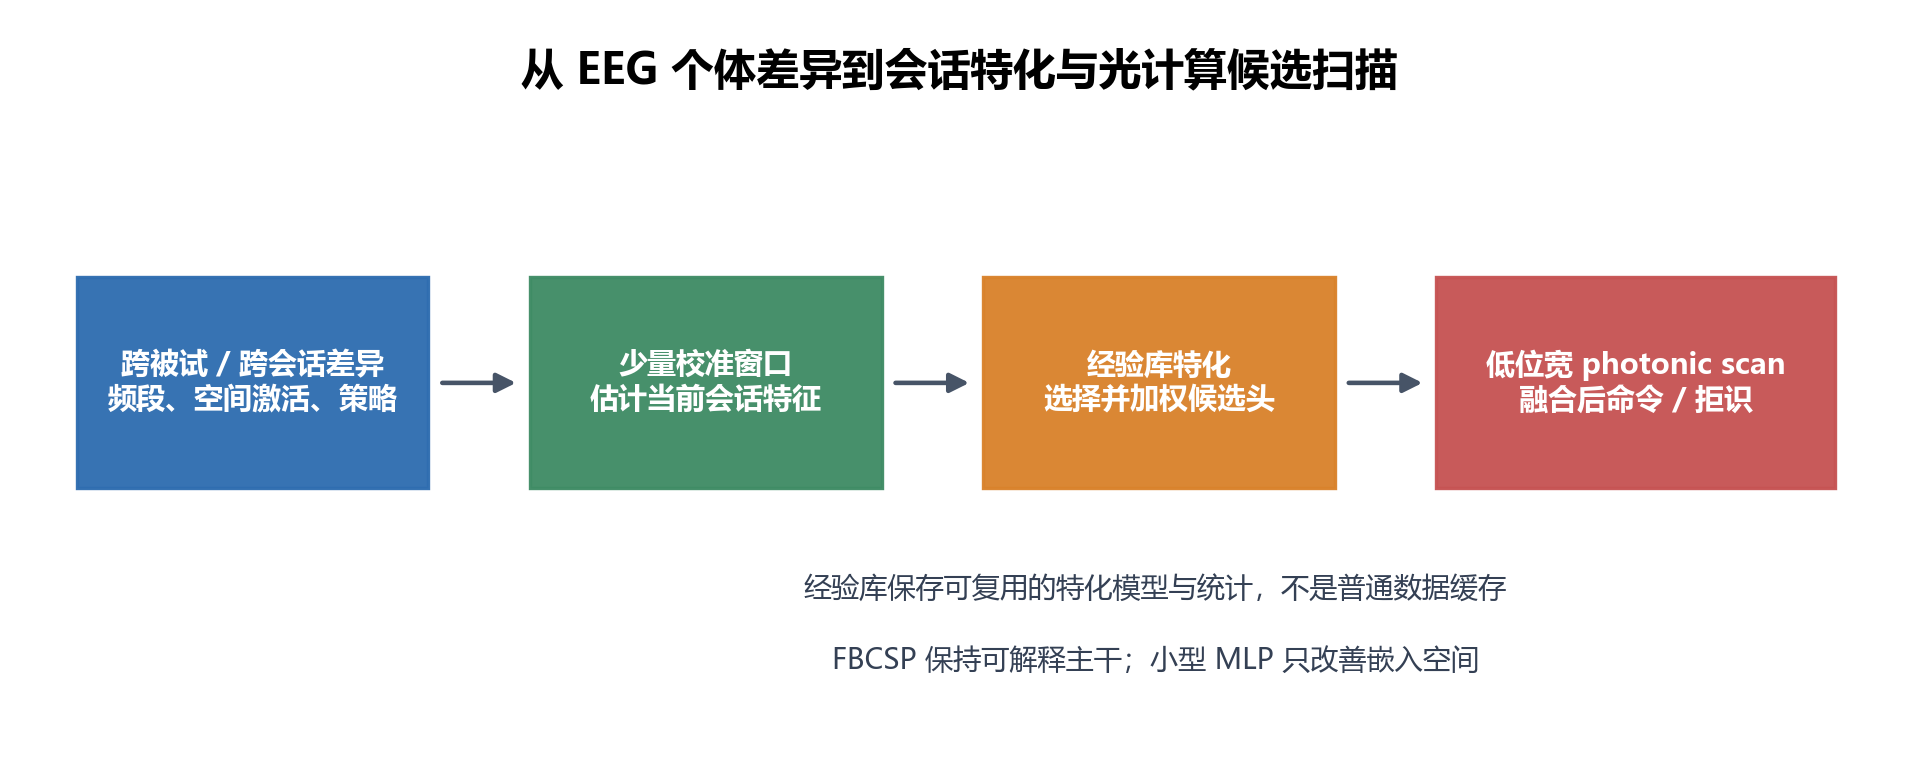
\includegraphics[width=0.94\linewidth]{competition/specialization_logic.png}
\caption{背景逻辑图：EEG 个体/会话差异推动少量校准和经验库特化，随后由低位宽候选扫描完成当前窗口的个性化判别。该图为方案逻辑说明。}\label{fig:specialization-logic}
\end{figure}

\section{方案主干与光电计算分工}
FBCSP（滤波器组公共空间模式）是运动想象 EEG 中稳定、可解释且对小样本友好的经典方法\cite{ang2012fbcsp,blankertz2008}。它在多个运动相关频带上学习空间投影，再以对数方差形成判别特征。本项目不把 FBCSP 只作为陪衬 baseline，而是把它作为系统主干：频带和空间滤波具有明确生理含义，也便于检查训练/测试数据边界。

FBCSP 同时包含滤波、空间投影 $Z=WX$、协方差或 Gram 矩阵等大量线性计算，天然适合对接矩阵/向量运算接口。深度学习只承担 32--64--32 的小型 embedding 模块，用来改善 FBCSP 特征空间中的会话表示和经验检索，不完全替代 FBCSP，也不把系统描述为纯深度学习 BCI。

当前工程采用 forward-only 统计口径：前向传播中的线性计算通过三个后端接口进入光计算接管路径，即 \texttt{MatrixOps}\allowbreak\texttt{Backend}、\texttt{SignalOps}\allowbreak\texttt{Backend} 和 \texttt{TiledMVM}\allowbreak\texttt{Backend}；候选线性头扫描是其中重点验证的 4-bit、$2\times8$ tile 量化路径。这里的“接管”只针对前向线性计算；激活、方差、对数、softmax、质量控制、拒识判断和经验库管理仍由数字端完成，候选概率的加权求和则作为线性组合进入 MatrixOps。因而光计算没有替代全部算法，而是在保留数字控制逻辑的前提下承接适合矩阵/向量实现的线性算子。

\section{项目目标与系统输出}
项目目标是构建一套由 FBCSP 主导、经验库增强并可接光计算后端的 MI-BCI 原型。工程同时保留 FBCSP + shrinkage LDA、FBCSP + small MLP embedding 和“FBCSP + embedding + 经验库 + photonic scan”三条实验线，用统一划分比较各模块作用；数据加载、训练、校准、评估、指标保存、绘图和进度记录均提供可复现入口。实时采集和 Cyton 上位机仅作为扩展目标，目前尚未完成真实 EEG 在线闭环。

系统标签仍是 left、right、foot 三个运动想象类别；reject 是推理阶段额外产生的安全状态，不是数据集原生第四类。当最高概率低于阈值、前两类概率间隔不足或信号质量不合格时，系统输出 reject，避免在意图不明确、注意力变化或伪迹窗口上误触发控制命令。因此本报告所称“四种输出”是“三个 MI 命令 + 一个系统拒识状态”，不能解释为四分类训练。

\begin{table}[H]
\centering\small
\renewcommand{\arraystretch}{0.95}
\caption{项目完成情况与可展示材料}\label{tab:status}
\begin{tabularx}{0.95\linewidth}{|L{0.25\linewidth}|L{0.19\linewidth}|X|}\hline
模块 & 状态 & 可在复赛中出示的证据 \\ \hline
FBCSP、MLP、经验库、拒识 & 已完成 & 单元测试、配置、JSON 指标、图\ref{fig:system}、图\ref{fig:fbcsp-flow}与图\ref{fig:mainline-confusion} \\ \hline
Cyton 上位机与模拟流 & 未完成 & 仅有 BrainFlow 适配器、串口参数、SQLite 经验组和 Tk 界面模块，尚未形成稳定在线闭环 \\ \hline
$2\times8$ tile 扫描 & 已完成光计算模拟器验证 & 分块累加实现、tile 计数、模拟器输出与浮点参考的一致性测试 \\ \hline
Gazelle 模拟器接口 & 已接通、性能待优化 & 单窗口运行识别到 gazelle\_simulator；已记录耗时与 tile 调度 \\ \hline
自适应精度优化 & 完善中（实验性） & 已实现 4/6/8-bit 单调升级、8-bit shadow 监测和初步 A/B；策略、阈值与算子覆盖尚未定版 \\ \hline
实时在线演示 & 未完成 & 当前核心证据来自公开数据回放；真实采集、质量门控、推理和反馈仍待联调 \\ \hline
\end{tabularx}
\end{table}

\section{系统总览}
图~\ref{fig:system}按信号流动顺序展示系统。流程分为五部分：采集与对齐、预处理、特征与特化、候选评分、安全输出。每个框对应第 2 章中的一个或多个步骤。虚线表示信号质量不合格时直接拒识，实线表示正常分类流程。训练阶段只使用训练数据来确定滤波器、CSP、标准化参数、小型网络和经验条目；评估和在线阶段只使用固定参数，不能用当前评估窗口重新训练。图中紫色阶段突出候选头的低位宽 tile 扫描，但按当前 forward-only 账本，其他前向线性算子也通过统一后端进入光计算接管路径。
\begin{figure}[H]\centering
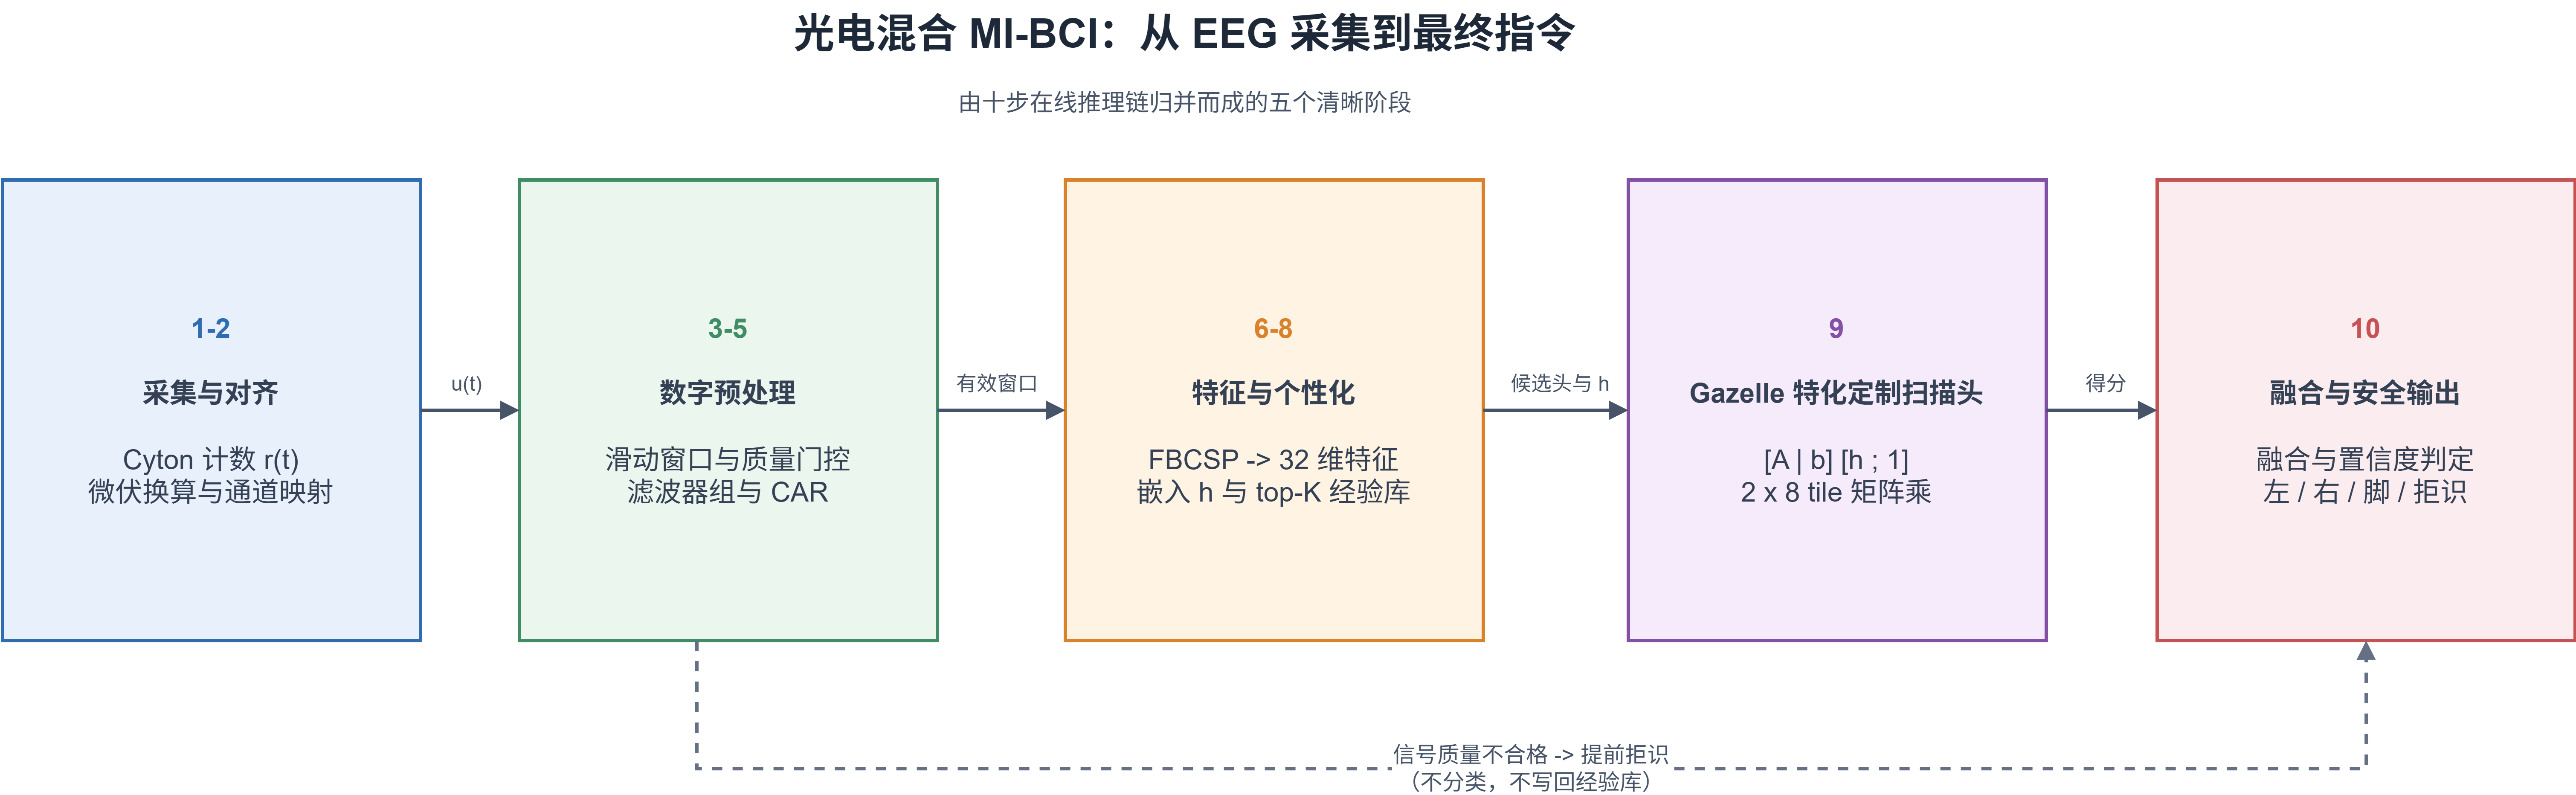
\includegraphics[width=0.98\linewidth]{competition/end_to_end_inference_chain.drawio.png}
\caption{光电混合 MI-BCI 从 EEG 采集到最终指令的简化结构。}\label{fig:system}
\end{figure}

\chapter{系统总体架构与算法路线}
\section{训练、校准与在线推理三个阶段}
三个阶段使用同一套 FBCSP、embedding、经验库和 backend 接口，但输入、允许更新的参数和输出不同。离线训练产生可部署模型，校准为新会话选择特化状态，在线推理只处理当前决策窗口。训练集、校准集和评估集严格隔离。

\subsection{离线训练阶段}
\subsubsection{第 1 步：加载训练数据并固定协议}
公开数据按被试、session 和 trial 形成训练集合；此时固定通道映射、事件窗口、采样率和 left/right/foot 全局标签。Evaluation windows 不参与任何拟合。训练输入为 $\{(X_n,y_n)\}_{n=1}^{N_{\mathrm{train}}}$，输出是可重复的数据划分与预处理配置。

\subsubsection{第 2 步：拟合滤波器组和 OVR CSP}
训练窗口经过 CAR 和 8--32 Hz 六频带滤波。对每个频带 $b$ 和类别 $k$ 估计收缩协方差，并求得 $W_{b,k}\in\mathbb{R}^{4\times C}$。由 $Z_{b,k}=W_{b,k}X_b$ 的归一化对数方差形成 72 维原始 FBCSP 特征。滤波器、CSP 和收缩参数在训练结束后冻结。

\subsubsection{第 3 步：选择特征并拟合标准化}
仅用训练标签计算 Fisher 分数，保存前 32 维索引集合 $\mathcal I$；随后估计训练特征均值 $\mu$ 和尺度 $\sigma$。部署时使用
\begin{equation}
x=f_{\mathrm{raw}}[\mathcal I],\qquad \bar{x}_d=\frac{x_d-\mu_d}{\sigma_d+\epsilon},
\end{equation}
不能在校准或评估窗口上重新选择特征或重估全局标准化参数。

\subsubsection{第 4 步：训练 baseline 与小型 embedding}
第一条线在 $\bar{x}$ 上拟合 shrinkage LDA。第二条与主线训练 $32\rightarrow64\rightarrow32$ 小型 MLP：
\begin{equation}
h_1=\phi(W_1\bar{x}+b_1),\qquad h=W_2h_1+b_2.
\end{equation}
网络只改善 FBCSP 特征空间，不替代前端。训练完成后导出 embedding 参数、直接分类头和训练阈值；训练与反向传播属于 setup，不计入单窗口 forward。

\subsubsection{第 5 步：建立初始经验库并保存部署包}
经验库包含全局 MLP anchor head、全局 embedding LDA head 和 64 个 bootstrap LDA heads。每个条目保存 entry id、centroid、linear head、source、训练索引和训练质量。训练阶段最终输出 FBCSP 参数、特征索引、标准化参数、MLP、经验库、类别顺序、量化配置和版本信息。

\subsection{校准阶段}
\subsubsection{第 1 步：输入少量目标会话窗口}
新被试或新 session 提供少量带标签或受控提示窗口。BCICIV 主线使用 42 个校准窗口；BNCI 对每位目标被试使用 session 3 中每类前 8 个 trial。校准窗口只用于查询和加权候选，不计入最终 evaluation 指标。

\subsubsection{第 2 步：用冻结主干生成 calibration embeddings}
校准窗口沿训练阶段冻结的滤波器、CSP、特征索引、标准化和 MLP 前向，得到 $h_j$。取其均值 $\bar h$ 作为当前会话查询表示，并计算经验条目距离
\begin{equation}
d_i=\|\bar h-e_i\|_2^2.
\end{equation}
该阶段不能重新训练 FBCSP 或 MLP，否则会破坏训练/评估边界。

\subsubsection{第 3 步：选择 top-$K$ 候选并计算融合权重}
候选集合固定保留两个全局 anchors，再按距离补足到 top-$K=8$。记训练准确率、校准准确率、校准真实类别置信度和锚点标记分别为 $a_i,c_i,u_i,r_i$，当前权重为
\begin{equation}\label{eq:retrieval-weight}
z_i=-0.25\tilde d_i+0.75a_i+3c_i+5r_i+0.5u_i,
\qquad
\alpha_i=\frac{\exp(z_i)}{\sum_{j\in\mathrm{top}\text{-}K}\exp(z_j)}.
\end{equation}
因此经验库是特化模型集合，不是样本缓存；没有校准数据时只能退回全局 anchor，并标记为未个性化。

\subsubsection{第 4 步：确定拒识阈值并冻结会话状态}
系统根据训练/校准分数确定置信度阈值 $\tau_p$ 和边际阈值 $\tau_m$，保存候选 head bank、权重、阈值、模型版本和会话元数据。校准输出是一次部署状态，不是控制命令，也不计入单窗口在线时延。

\subsection{在线推理阶段}
\subsubsection{第 1 步：形成一个 EEG 决策窗口}
公开数据回放直接读取已切分 trial $X\in\mathbb{R}^{C\times T}$。实采目标从 Cyton 样本序号、时间戳和 ADC 计数开始，以 $u_{c,t}=g r_{c,t}$ 换算微伏并写入环形缓冲区：
\begin{equation}\label{eq:windowing}
X^{(m)}=\left[u_{c,t}\right]_{c=1:C,\;t=t_m-T+1:t_m}.
\end{equation}
在线目标窗口为 2.0 s、步长为 0.5 s；真实 Cyton 连续采集链尚未完成闭环。

\subsubsection{第 2 步：质量检查与提前拒识}
对每个通道检查标准差、最大幅值、相邻跳变、工频/肌电功率比和坏通道比例。质量标记 $q^{(m)}=1$ 时直接输出“信号质量不足”，不继续分类也不写入经验库。该质量门控是在线扩展目标；当前回放主要验证分类置信度拒识。

\subsubsection{第 3 步：滤波、CAR 与 FBCSP transform}
有效窗口经过高通、陷波、六频带滤波和有效通道 CAR。在线 IIR 需保存历史状态；回放使用既定零相位处理。冻结的空间滤波器执行
\begin{equation}
Z_{b,k}=W_{b,k}X'_b,qquad
f_{b,k,r}=\log\frac{\operatorname{var}(Z_{b,k,r,:})}{\sum_j\operatorname{var}(Z_{b,k,j,:})+\epsilon},
\end{equation}
再按固定 $\mathcal I$ 得到 32 维特征。当前窗口不能重新拟合 CSP 或重选特征。

\subsubsection{第 4 步：标准化并生成 embedding}
使用训练阶段保存的 $\mu,\sigma,W_1,W_2$ 得到 $\bar{x}$ 和 32 维 $h$。推理关闭 dropout；$h$ 是候选头输入，不是最终概率。标准化和 MLP 线性层通过 MatrixOps backend，激活仍在数字端。

\subsubsection{第 5 步：量化并扫描候选线性头}
每个候选包含 $A_i\in\mathbb{R}^{3\times32}$ 和 $b_i\in\mathbb{R}^{3}$：
\begin{equation}\label{eq:e2e-candidate}
s_i=[A_i\;b_i]\begin{bmatrix}h\\1\end{bmatrix}\in\mathbb{R}^{3}.
\end{equation}
\texttt{TiledMVM}\allowbreak\texttt{Backend} 将 $3\times33$ 增广矩阵按 $2\times8$ tile 切分。一个候选需 $2\times5=10$ 次、8 个候选共 80 次 tile。最新单窗口运行已加载 Gazelle 模拟器：候选路径为 \texttt{gazelle}\allowbreak\texttt{\_simulator}，其他线性路径为 \texttt{gazelle}\allowbreak\texttt{\_simulator}\allowbreak\texttt{\_bit}\allowbreak\texttt{\_sliced}；这仍是模拟器结果，不是真实芯片实测。

\subsubsection{第 6 步：融合、平滑、拒识并输出命令}
候选得分经 softmax 后按校准权重融合：
\begin{equation}
\pi_{i,k}=\frac{\exp(s_{i,k})}{\sum_j\exp(s_{i,j})},\qquad
p_k=\sum_{i=1}^{K}\alpha_i\pi_{i,k}.
\end{equation}
可对相邻窗口做指数平滑 $\widetilde p^{(m)}=\rho p^{(m)}+(1-\rho)\widetilde p^{(m-1)}$。最终决策为
\begin{equation}\label{eq:final-decision}
\hat y=\begin{cases}
\mathrm{reject}, & q^{(m)}=1\ \text{或}\ \max_k\widetilde p_k<\tau_p\ \text{或}\ \widetilde p_{(1)}-\widetilde p_{(2)}<\tau_m,\\
\arg\max_{k\in\{\mathrm{left,right,foot}\}}\widetilde p_k, & \text{其他情况}.
\end{cases}
\end{equation}
回放模式同时累计准确率和拒识率；真实在线只能显示命令、概率、置信度、质量和拒识原因，不能显示无真值的实时准确率。

\section{公开数据回放与实采在线模式}
当前核心实验采用公开数据回放：输入是数据集已经切分并带真值标签的 trial，因此可以计算 command accuracy、balanced accuracy、accepted accuracy、reject rate、rolling 和 cumulative 指标。实采在线模式的目标输入是 Cyton 连续数据包，还需要丢包检查、ADC 换算、环形缓冲区、窗口切片和信号质量门控；该路径尚未形成稳定闭环。两种模式在形成决策窗口后共享 FBCSP、embedding、经验库、photonic scan 和拒识逻辑，但真实在线没有即时真值，不能显示“实时准确率”。

\section{三条算法实验线}
第一条 baseline 为 FBCSP + shrinkage LDA。它使用多频带 OVR CSP、对数方差、Fisher 特征选择和收缩 LDA，强调小样本稳定性与可解释性。第二条为 FBCSP + small MLP embedding：输入仍是筛选后的 FBCSP 特征，小网络增加非线性表示并直接输出分类结果，但尚未使用经验库。主线在第二条基础上加入经验库检索、top-$K$ 候选头和低位宽 photonic scan，用少量校准实现会话特化。三条线使用相同训练/评估边界，以免把数据划分差异误当成模块收益。

\section{两级拒识机制}
第一级是分类前的质量拒识：检查平线、饱和、突变、坏通道以及工频/肌电干扰，不合格窗口不继续分类，也不写入经验库。第二级是分类后的置信度拒识：当最高概率或前两类概率边际不足时输出 reject。前者处理不可用信号，后者处理模型不确定性，共同降低外部控制误触发。当前公开数据回放完整验证了第二级拒识；第一级质量门控仍属于在线上位机联调内容。

\section{数据、窗口与质量控制}
原型的目标通道为运动区附近的 8 个电极 $\{\mathrm{C3,C4,Cz,FC3,FC4,CP3,CP4,CPz}\}$。公开数据实验按各数据集提供的通道和事件定义进行。在线目标使用 $T_w=2.0\,\mathrm{s}$ 的窗口，每 $0.5\,\mathrm{s}$ 更新一次，兼顾稳定性和输出速度。离线实验不重新切分 trial，而是直接使用数据集事件窗：BCICIV\_1\_asc 为 marker 后 1.0--4.0 s，BNCI2014\_004 为 0.5--3.5 s。输入窗口记为 $X\in\mathbb{R}^{C\times T}$，其中 $C=8$，$T$ 由采样率和实验设置决定。

每个窗口先检查坏通道、饱和、幅值突变、工频和高频肌电干扰。若质量分数 $q$ 超过阈值，只输出拒识，这个窗口也不会写回经验库。对有效通道 $\mathcal{V}$ 使用公共平均参考（CAR）：
\begin{equation}\label{eq:car}
X'_{c,t}=X_{c,t}-\frac{1}{|\mathcal{V}|}\sum_{j\in\mathcal{V}}X_{j,t}.
\end{equation}
之后使用 $0.5\,\mathrm{Hz}$ 高通、$50\,\mathrm{Hz}$ 陷波和六个三阶 SOS 带通（8--12、12--16、16--20、20--24、24--28、28--32 Hz）。离线实验使用零相位滤波，保证与原始数据处理方式一致；在线版本使用保留状态的因果滤波器，并单独检查结果变化。

\section{滤波器组公共空间模式（FBCSP）}
FBCSP 会分别处理多个频带。对每个频带 $b$ 和类别 $k$，把该类别和其余类别分开，计算归一化协方差 $\Sigma_{b,k}$ 与 $\Sigma_{b,\neg k}$。为避免训练数据较少时结果不稳定，使用收缩后的协方差：
\begin{equation}
\widetilde{\Sigma}=(1-\lambda)\Sigma+\lambda\frac{\operatorname{tr}(\Sigma)}{C}I,
\end{equation}
其中 $\lambda=0.15$。接着求 CSP 空间滤波器 $w$：
\begin{equation}\label{eq:csp}
\widetilde{\Sigma}_{b,k}w=\gamma(\widetilde{\Sigma}_{b,k}+\widetilde{\Sigma}_{b,\neg k})w.
\end{equation}
每个类别任务保留两端各两条空间滤波器，得到 $Z_{b,k}=W_{b,k}X'_b$。再计算这些信号的归一化对数方差：
\begin{equation}\label{eq:fbcsp}
f_{b,k,r}=\log\frac{\operatorname{var}(Z_{b,k,r})}{\sum_j\operatorname{var}(Z_{b,k,j})+\epsilon}.
\end{equation}
六个频带、三个类别任务、每个任务四条滤波器，一共得到 72 维原始 FBCSP 特征。Fisher 分数 $J_d$ 只用训练数据计算，并选出前 32 维：
\begin{equation}
J_d=\frac{\sum_k n_k(\mu_{k,d}-\mu_d)^2}{\sum_k n_k\sigma_{k,d}^{2}+\epsilon}.
\end{equation}
这样可以看出哪些频段和空间方向对分类有帮助，同时把主要计算集中到矩阵投影上。

图~\ref{fig:fbcsp-flow}展示了 FBCSP 如何把多通道 EEG 变成紧凑特征。滤波、方差和对数不属于矩阵乘；每个频带和每个类别任务中的 $Z=W X$ 才是标准矩阵乘。若把 $W\in\mathbb{R}^{4\times8}$ 按 $2\times8$ tile 切分，每个采样时刻需要 $\lceil4/2\rceil\lceil8/8\rceil=2$ 次 tile 计算。6 个频带、3 个类别任务、$T$ 个采样点共需要 $36T$ 次。这个数量较大，因此本项目先把候选线性头作为重点仿真对象。
\begin{figure}[H]\centering
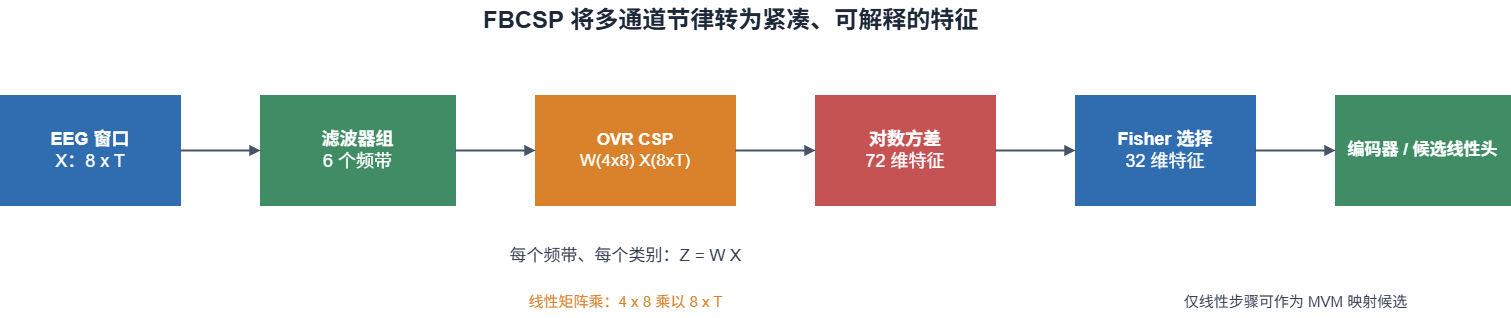
\includegraphics[width=0.96\linewidth]{competition/fbcsp_matrix_flow.drawio.png}
\caption{FBCSP 的数据流和线性热点。CSP 投影 $W(4\times8)X(8\times T)$ 是可拆分为 tile 的矩阵乘；log-variance 与特征选择保留在数字端。}\label{fig:fbcsp-flow}
\end{figure}

\section{小型嵌入网络与经验库}
选出的 32 维特征 $x\in\mathbb{R}^{32}$ 先按训练集的均值和标准差做标准化：$\bar{x}_d=(x_d-\mu_d)/(\sigma_d+\epsilon)$。之后进入一个 $32\rightarrow64\rightarrow32$ 的小网络：
\begin{equation}\label{eq:encoder}
h=W_2\,\phi\left(W_1\bar{x}+b_1\right)+b_2,\qquad h\in\mathbb{R}^{32},
\end{equation}
其中 $\phi$ 是 GELU 或 ReLU 激活函数，训练时使用 dropout。这个小网络不直接替代前面的信号处理，而是把当前窗口变成便于和历史记录比较的嵌入向量。

推理时，标准化也能写成矩阵形式 $\bar{x}=D x+c$，把常数项合并后就是 $[D\;c][x;1]$。因此，标准化、第一层和第二层的矩阵大小分别为 $32\times33$、$64\times33$、$32\times65$；对应的 $2\times8$ tile 数分别为 80、160、144。这些层和候选扫描都可以按相同的量化、切块和累加规则在 LTSimulator 中计算。

每条经验记录会保存设备和通道信息、预处理版本、CSP 参数、选出的特征、标准化参数、编码器版本、嵌入中心、线性头和拒识阈值。对新会话的少量校准窗口，计算
\begin{equation}
d_i=\left\|\frac{1}{n}\sum_{j=1}^{n}h_j-e_i\right\|_2^2
\end{equation}
来找 top-$K$ 条最相近的经验。候选模型必须来自历史训练、bootstrap 或受控微调，不能随意用随机权重生成。只有准确率、拒识率和质量指标都满足要求时，才把该会话写回经验库。

\section{候选扫描、融合与拒识}
每个候选线性头包含 $A_i\in\mathbb{R}^{3\times32}$ 和 $b_i\in\mathbb{R}^{3}$。加上常数通道后，可以把得分写成一次矩阵乘：
\begin{equation}\label{eq:scan}
s_i=\left[A_i\;b_i\right]\begin{bmatrix}h\\1\end{bmatrix},\quad i=1,\ldots,K.
\end{equation}
再按检索权重 $\alpha_i$ 合并各候选的概率：
\begin{equation}
p=\sum_{i=1}^{K}\alpha_i\operatorname{softmax}(s_i),\qquad \sum_i\alpha_i=1.
\end{equation}
如果最高概率 $\max_k p_k$ 太低、前两类概率差 $p_{(1)}-p_{(2)}$ 太小，或质量检测发现伪迹，就输出 ``拒识''；否则输出概率最大的类别 $\arg\max_kp_k$。这样能减少低质量信号被误当成控制指令的情况。

\chapter{光计算接口、量化与计算统计}
\section{统一后端接口}
三个接口按计算层次分工：MatrixOps 处理通用矩阵运算，SignalOps 处理具有时间轴和滤波状态的 EEG 线性操作，TiledMVM 处理候选矩阵 bank 的分块扫描。上层 FBCSP、embedding 和经验库只依赖抽象接口，不直接调用某个硬件驱动。

\subsection{MatrixOpsBackend：通用矩阵运算接口}
\texttt{MatrixOps}\allowbreak\texttt{Backend} 的基础契约是
\begin{center}\small
\path{matmul(left, right, name) -> array}\\
\path{einsum(subscripts, operands, name) -> array}
\end{center}
输入可以是向量、矩阵或批量张量，输出保持与 NumPy 线性代数一致的 shape；\texttt{name} 为每个算法算子保留可读标识，便于驱动路由、调用记录和 compute accounting。仿射变换通过在输入末尾拼接常数 1 转换为矩阵乘，距离计算和候选概率融合中的点积也通过同一接口表达。

当前通过 MatrixOps 路由的主要步骤包括：FBCSP/CSP 空间投影与协方差乘积、特征标准化仿射、MLP 前向线性层、LDA 参数与分类分数、经验库 centroid 距离交叉项以及候选概率线性融合。激活、方差、对数、softmax、阈值和矩阵分解不属于该接口。\texttt{NumpyMatrixOpsBackend} 仅保留为开发调试参考；正式前向实验通过 photonic backend 调用光计算模拟器，完成量化、$2\times8$ tile 或 4-bit slice 拆分、模拟器读回、零点补偿和反量化。当前证据属于光计算模拟器验证，尚未替换为真实光芯片驱动。

\subsection{SignalOpsBackend：EEG 时序线性操作接口}
\texttt{SignalOps}\allowbreak\texttt{Backend} 将具有通道轴或时间轴语义的前向信号处理与普通矩阵乘分开，当前契约为
\begin{center}\small
\path{common_average_reference(samples, channel_axis, name)}\\
\path{sosfiltfilt(sos, samples, axis, name)}
\end{center}
CAR 接口沿指定通道轴减去有效通道平均值；SOS 接口沿指定时间轴执行滤波器组。显式的 axis 参数避免在 trial、channel、sample 维度变化时误处理数据，name 参数用于区分训练、校准和 evaluation 中的调用。

公开数据回放使用零相位 \texttt{sosfiltfilt}，便于与现有实验协议保持一致；真实在线需要保留滤波状态的因果 SOS 接口，不能直接使用未来采样点。当前 photonic SignalOps 仍是软件 stand-in，并按 MAC-equivalent 记入 forward-only 账本；这表示接口已接管，不表示 CAR 和整条 IIR 状态机已经在真实光芯片上执行。坏通道选择、伪迹判断和滤波状态管理仍属于数字控制逻辑。

\subsection{TiledMVMBackend：候选头 bank 扫描接口}
\texttt{TiledMVM}\allowbreak\texttt{Backend} 面向经验库选出的候选矩阵 bank，接口为
\begin{center}\small
\path{scan(weights, features) -> candidate_outputs}\\
\path{count_tiles(weights) -> tile_count}
\end{center}
其中 weights shape 为 $(N,M,D)$，表示 $N$ 个候选、每个候选 $M$ 个输出和 $D$ 维输入；features shape 为 $(D,)$；输出 shape 为 $(N,M)$。接口先检查维度匹配，再依次扫描候选、输出行块和输入列块，并把每个 tile 的部分和累加到对应候选输出。

主线把 8 个 $3\times33$ 增广候选头交给该接口。默认 tile 为 $2\times8$，所以一次 scan 需要 $8\lceil3/2\rceil\lceil33/8\rceil=80$ 次 tile。每个 tile 内部调用量化 MatrixOps backend；候选路径默认单次 4-bit，偏置作为常数输入一并扫描。\texttt{last\_tile\_count} 和 \texttt{count\_tiles} 提供调度证据。正式实验调用已加载的 Gazelle 光计算模拟器；代码中的数字矩阵乘只作为模拟器不可用时的开发调试回退，不作为报告结果来源。真实芯片的传输、标定和读回仍需未来驱动实现。

三个接口共同建立“算法 shape 不受物理 tile 限制”的边界。当前实验性方案中，候选扫描使用单次 4-bit；其他前向线性算子由自适应 bit-sliced backend 接管，CAR 从 4-bit 起步，SOS、FBCSP 投影和特征标准化从 6-bit 起步，未命中低位宽策略的敏感路径保持 8-bit。所有逻辑精度仍拆为 uint4/int4 物理调用，并允许低精度算子按误差监测结果单调升级至 6-bit 或 8-bit。该优化仍在完善，初始位宽、阈值、监测周期和算子覆盖不代表最终配置；同时必须继续区分 backend 路由、量化配置和真实芯片逐算子实测三个证据层次。

\section{候选扫描的设计动机}
\subsection{光计算单元与多候选 MVM 的匹配}
光计算单元的目标优势是以较高并行度和较低数据搬移开销完成矩阵/向量乘。对于单个固定分类头，矩阵规模较小，专门引入 tile 调度的收益有限；经验库特化则会在一次校准后保留 top-$K$ 个候选头，使同一个 EEG 决策窗口需要执行 $K$ 次结构完全相同、权重不同的 MVM。若逐个在通用数字路径上调用，计算和权重读取开销随 $K$ 近似线性增长；把这些头组织成规则的候选 bank，更符合光计算批量扫描线性算子的使用方式。

这里的低功耗和高并行是光计算平台的设计目标，不是本文已经测得的芯片结论。当前工程验证的是候选 MVM 的统一接口、量化、tile 数量和软件读回；真实能耗、吞吐与延迟仍需硬件实测。

\subsection{经验库检索与 Candidate head bank}
经验库不是普通样本缓存，而是由全局 anchors 和 bootstrap 特化模型组成的候选线性头集合。校准阶段根据 embedding 距离、训练质量、校准准确率、校准置信度和 anchor 先验选择 top-$K$，得到
\begin{equation}
\mathcal H_K=\{(A_i,b_i,\alpha_i)\}_{i=1}^{K},
\qquad A_i\in\mathbb{R}^{M\times D},\quad b_i\in\mathbb{R}^{M}.
\end{equation}
将偏置并入常数输入后，多个头可以堆叠为
\begin{equation}
\mathcal A=\operatorname{stack}\left([A_1\;b_1],\ldots,[A_K\;b_K]\right)
\in\mathbb{R}^{K\times M\times(D+1)},
\qquad \widetilde h=[h;1].
\end{equation}
因此经验库查询的输出不是一个模型，而是一个带检索权重 $\alpha_i$ 的 candidate head bank。主线取 $K=8$、$M=3$、$D=32$，即输入给 \texttt{TiledMVMBackend} 的 weights shape 为 $(8,3,33)$，features shape 为 $(33,)$。

\subsection{Candidate scores 与概率融合}
Photonic scan 对同一个 $\widetilde h$ 扫描整个 head bank，输出
\begin{equation}
S=\operatorname{scan}(\mathcal A,\widetilde h)
\in\mathbb{R}^{K\times M},\qquad s_i=[A_i\;b_i]\widetilde h.
\end{equation}
其中每一行 $s_i$ 是一个候选头对 left/right/foot 的分类分数，不是最终类别，也不是最终融合概率。数字端分别计算 $\pi_i=\operatorname{softmax}(s_i)$，再使用校准阶段得到的检索权重
\begin{equation}
p=\sum_{i=1}^{K}\alpha_i\pi_i,qquad \alpha_i\geq0,\quad\sum_i\alpha_i=1.
\end{equation}
最终命令还要经过时间平滑、最高概率阈值和前两类边际阈值。这样 photonic scan 负责规则、可批量的线性得分，数字端保留非线性概率解释、经验权重融合和安全拒识。

\subsection{决策路径重组与创新边界}
Photonic scan 的设计不是把原代码中的一次 \texttt{np.matmul} 简单换成另一个函数，而是利用 MI-EEG 个体差异先形成“少量校准 $\rightarrow$ 经验库检索 $\rightarrow$ 多候选线性头”，再把新增的多候选计算重组为规则 head bank 并交给 tiled MVM。算法特化产生并行候选，光计算接口承担候选扫描，两者共同构成主线设计逻辑。

本节所称 scan 是“一个 EEG 决策窗口内快速扫描多个候选校准器/线性头”。它不是 Goertzel 或其他频率扫描算法，也不在 8--30 Hz 上逐频点检测；频带处理已经由前面的滤波器组完成。它也不是只计算一个固定全局分类头：anchors 只是候选集合的一部分，最终结果来自 top-$K$ 候选分数和检索权重的融合。当前软件实现证明了 shape、4-bit 候选量化、$2\times8$ tile 调度和输出重构，尚未证明真实光芯片的并行度或能效收益。

\section{从算法矩阵到 \texorpdfstring{$2\times8$}{2x8} tile}
LTSimulator 中使用的基本计算块大小是 $R_t\times C_t=2\times8$，但算法里的矩阵通常更大。把任意 $A\in\mathbb{R}^{M\times D}$ 切成小矩阵 $A_{pq}$ 后，再由数字端把各块结果相加：
\begin{equation}\label{eq:tile}
Ax=\sum_{p=1}^{\lceil M/R_t\rceil}\sum_{q=1}^{\lceil D/C_t\rceil}A_{pq}x_q.
\end{equation}
因此 $K$ 个候选头的单窗口 tile 调用次数为
\begin{equation}\label{eq:tilecount}
N_{\mathrm{tile}}=K\left\lceil\frac{M}{2}\right\rceil\left\lceil\frac{D+1}{8}\right\rceil.
\end{equation}
主线使用 $K=8,M=3,D=32$。加上 bias 后，每个窗口需要 $8\times2\times5=80$ 次 tile 计算。图~\ref{fig:tiles}展示了这一过程。这里的 ``2x8'' 只表示 tile 的大小，不限制 FBCSP 特征的维数。
\begin{figure}[H]\centering
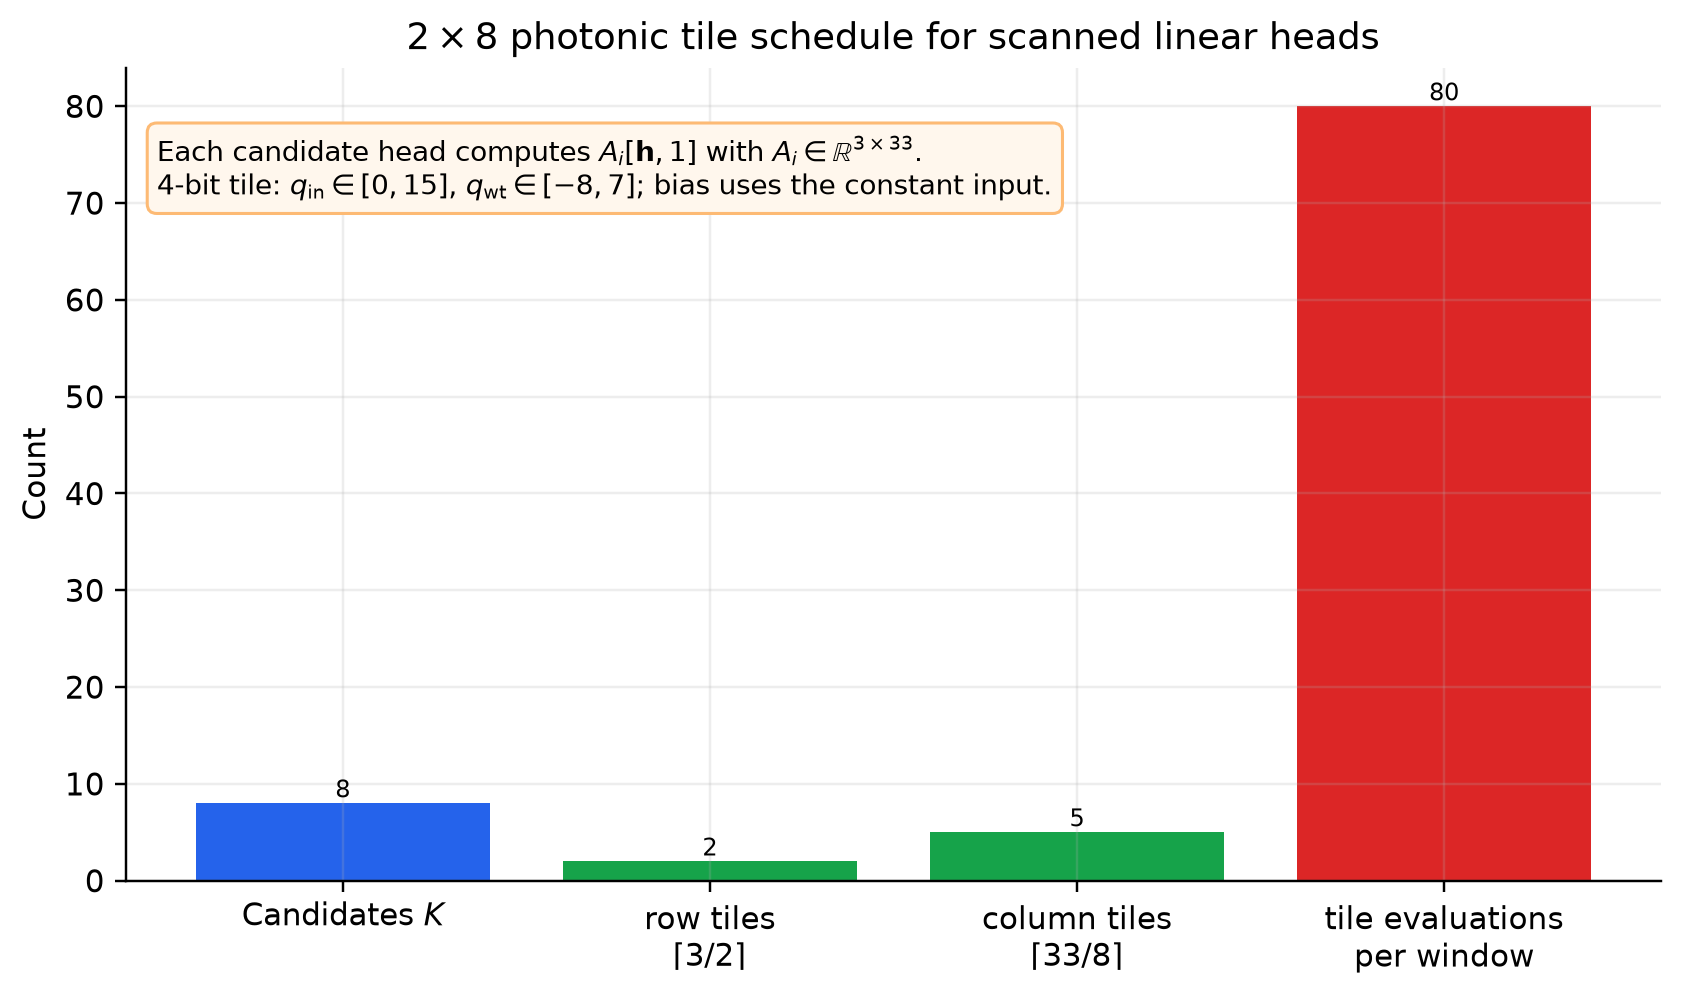
\includegraphics[width=0.90\linewidth]{competition/tile_schedule.png}
\caption{每个决策窗口的候选线性头 tile 调度。数字端负责跨 tile 部分和累加、softmax、拒识和融合。}\label{fig:tiles}
\end{figure}

图~\ref{fig:photonic-mapping}进一步说明式~\eqref{eq:scan}怎样切块。33 列输入包括 32 维嵌入向量和一个常数 1；最后一列所在 tile 的空位补 0。3 行输出分成两组 tile，第二组只有一行有效数据。每个候选需要 $2\times5=10$ 次 tile，8 个候选共需 80 次。数字端负责把各列的部分结果相加，再完成概率融合和拒识。
\begin{figure}[H]\centering
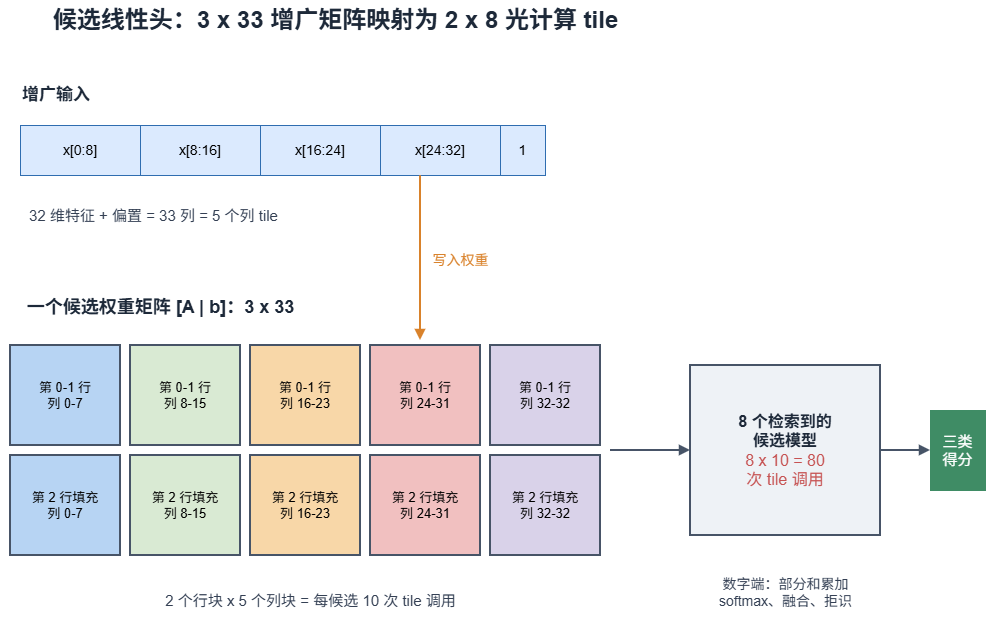
\includegraphics[width=0.97\linewidth]{competition/photonic_tile_mapping.drawio.png}
\caption{候选线性头的 $3\times33\rightarrow2\times8$ 映射概念图。颜色表示列分块；图示为一次候选扫描的计算拆分。}\label{fig:photonic-mapping}
\end{figure}

\section{逐算子矩阵乘拆分}
为了能复查光计算比例，我们不只看模块名称，而是逐个列出实际的线性计算。表~\ref{tab:matrix-split}给出主线单个窗口的拆分方式。``接管'' 表示矩阵大小已按统一接口和 tile/slice 规则执行并写入账本；真实芯片结论仍需补充硬件调用、读回结果、量化配置和日志。
\begin{table}[H]\centering\small
\caption{主线算法到光子矩阵乘的拆分}\label{tab:matrix-split}
\begin{tabularx}{0.96\linewidth}{|L{0.17\linewidth}|L{0.27\linewidth}|L{0.18\linewidth}|Y|}\hline
算法步骤 & 矩阵表达式与大小 & $2\times8$ tile 数 & 当前处理建议 \\ \hline
CAR 重参考 & $X'=(I-\frac1C\mathbf{1}\mathbf{1}^\top)X$，$8\times8$ 乘 $8\times T$ & $4T$ & SignalOps 展开后由 adaptive MatrixOps 接管，4-bit 起步 \\ \hline
SOS 滤波状态 & $s_{n+1}=As_n+Bx_n$，$y_n=Cs_n+Dx_n$ & 按频带、通道、section 和 direction 逐样本调度 & SignalOps 展开后由 adaptive MatrixOps 接管，6-bit 起步 \\ \hline
OVR CSP 投影 & $Z=W X$，$4\times8$ 乘 $8\times T$ & $2T$/频带/类别 & MatrixOps 接管；每个频带和类别独立监测，6-bit 起步 \\ \hline
特征标准化 & $[D\;c][x;1]$，$32\times33$ 乘 $33\times1$ & 80 & MatrixOps 仿射接管，6-bit 起步 \\ \hline
MLP 编码器 & $W_1[\bar{x};1]$：$64\times33$；$W_2[h_1;1]$：$32\times65$ & 160 + 144 & MatrixOps 接管并保持 8-bit；GELU/dropout 在数字端计算 \\ \hline
候选线性头 & $[A_i\;b_i][h;1]$，$8$ 个 $3\times33$ 乘 $33\times1$ & \textbf{80} & TiledMVM 接管；规则、批量、单次 4-bit \\ \hline
候选融合 & $p=\alpha^\top P$，$1\times8$ 乘 $8\times3$ & 2 & MatrixOps 以 8-bit 线性组合接管；softmax 和拒识留在数字端 \\ \hline
\end{tabularx}
\end{table}

\section{量化策略}
\subsection{两层位宽口径与当前支持}
本文区分“算法逻辑精度”和“物理单次调用位宽”。逻辑精度描述上层算子希望保留的定点动态范围；物理位宽描述一次 photonic tile 调用实际接收的整数范围。当前物理契约固定为
\begin{equation}
q_x^{(s)}\in[0,15]\quad(\mathrm{uint4}),
\qquad q_w^{(s)}\in[-8,7]\quad(\mathrm{int4}).
\end{equation}
候选 head scan 直接采用一次 4-bit 量化调用。其他前向线性路径采用 4/6/8-bit 自适应逻辑精度，再拆成 uint4/int4 slice 重构；因此“6-bit 或 8-bit 逻辑精度”不表示一次原生 uint6/int6 或 uint8/int8 光计算调用。固定 8-bit bit-sliced 路径作为数值对照基线保留。

\begin{table}[H]\centering\small
\caption{当前前向线性算子的量化策略}\label{tab:quant-policy}
\begin{tabularx}{0.96\linewidth}{|L{0.29\linewidth}|L{0.25\linewidth}|X|}\hline
算子路径 & 逻辑精度 & 物理调用 \\ \hline
CAR & 4-bit 起步，可升级至 6/8-bit & uint4/int4 slice；每次调用监测 \\ \hline
SOS 状态转移 & 6-bit 起步，可升级至 8-bit & uint4/int4 slices；首调用及每 64 次监测 \\ \hline
FBCSP 投影、标准化 & 6-bit 起步，可升级至 8-bit & uint4/int4 slices；每次调用监测 \\ \hline
MLP、LDA、距离交叉项、概率融合 & 8-bit & uint4/int4 slices \\ \hline
候选 head bank scan & 4-bit & 单次 uint4/int4 tiled MVM \\ \hline
\end{tabularx}
\end{table}

\subsection{单次 4-bit 量化配置}
对一个待计算 tile，输入 activation 使用仿射无符号量化。设输入范围为 $[x_{\min},x_{\max}]$，$Q_x=15$，则
\begin{equation}\label{eq:quant}
\begin{aligned}
s_x&=\frac{x_{\max}-x_{\min}}{Q_x},\\
z_x&=\operatorname{clip}\left(\operatorname{round}\left(-\frac{x_{\min}}{s_x}\right),0,Q_x\right),\\
q_x&=\operatorname{clip}\left(\operatorname{round}\frac{x}{s_x}+z_x,0,15\right).
\end{aligned}
\end{equation}
权重使用有符号对称量化。令 $Q_w=7$，则 $s_w=\max|W|/Q_w$，并取
\begin{equation}
q_w=\operatorname{clip}\left(\operatorname{round}(W/s_w),-8,7\right).
\end{equation}
整数乘积读回后先减去输入零点造成的偏移，再乘 $s_xs_w$ 反量化。偏置作为常数 1 的增广输入进入同一矩阵乘。4-bit 是当前重点验证位宽，用于在动态范围、调用复杂度和潜在硬件效率之间建立可实现基线；其抗噪和能效优势仍需真实器件测试。

候选扫描是当前真正的单次低位宽路径：每个 $2\times8$ tile 只进行一次 uint4/int4 乘加，不再用额外 slice 恢复更高逻辑精度。工程记录量化范围、scale、zero point、tile 数和反量化输出，用浮点参考检查分类分数偏差。

\subsection{Radix-16 位权拆分与 4/6/8-bit 逻辑精度}
普通前向线性路径按算子敏感度选择逻辑动态范围。无符号输入整数按 radix-16 展开为
\begin{equation}
q_x=\sum_{i=0}^{S_x-1}16^i q_{x,i},\qquad q_{x,i}\in[0,15],
\end{equation}
有符号权重使用 balanced radix-16 digits：
\begin{equation}
q_w=\sum_{j=0}^{S_w-1}16^j q_{w,j},\qquad q_{w,j}\in[-8,7].
\end{equation}
于是逻辑整数乘可由多个物理 slice 对重构：
\begin{equation}
q_xq_w=\sum_{i=0}^{S_x-1}\sum_{j=0}^{S_w-1}16^{i+j}\left(q_{x,i}q_{w,j}\right).
\end{equation}
矩阵先按输出 2 行、输入 8 列拆成物理 tile，每个 tile 再遍历输入/权重 slice 对；数字端按 $16^{i+j}$ 累加 partial sums，最后做零点补偿和反量化。因此一次逻辑 MVM 的物理调用数约为“空间 tile 数 $\times S_xS_w$”，不能只报告算法矩阵的一次调用。

这种 positional decomposition 可以保留 6-bit 或 8-bit 逻辑精度，区别于把高位宽值直接截断为 4-bit。代价是更多 slice 调用、部分和累加、潜在噪声传播和更高延迟；4-bit 路径只需要一个物理 slice，6-bit 和 8-bit 路径则按位权拆分后重构。

\subsection{当前实验性实现与证据边界}
通用 MatrixOps 路径当前由 \texttt{AdaptivePrecision}\allowbreak\texttt{PhotonicMatrixOps}\allowbreak\texttt{Backend} 接管，physical slice bits 固定为 4。SignalOps 中 CAR 展开为通道混合矩阵；SOS 的二阶节用状态转移形式表达，其系数乘加调用同一 adaptive bit-sliced MatrixOps 路径。FBCSP 每个频带、SOS section、direction 和 CSP 类投影分别维护精度状态；候选 scan 则由 \texttt{QuantizedPhotonic}\allowbreak\texttt{MatrixOpsBackend} 完成单次 4-bit tile 计算。

低于 8-bit 的算子在首次调用及策略规定的周期上，与数字端模拟的 8-bit bit-sliced shadow 输出比较归一化误差。误差超过该算子的阈值时，本次调用立即按下一档位宽重新计算，并将该具体算子永久升级；精度不会自动下降。CAR、SOS、FBCSP 投影和标准化的当前实验误差上限分别为 0.03、0.06、0.05 和 0.04，这些数值尚未定版。运行时保存每个算子的当前位宽、监测次数、最大误差、升级次数和 tile 数，便于后续调整精度与资源开销。

当前量化在运行时根据张量范围动态计算 scale 和 zero point，并进行位权拆分；这不是量化感知训练（QAT）。只有后续实验表明小型 MLP 或其他敏感算子的低位宽误差显著破坏 command accuracy、accepted accuracy 或 reject rate 时，才考虑在训练中加入 fake quantization/QAT。

正式前向实验通过 Gazelle 光计算模拟器执行。本开发环境无法直接调用该模拟器，因此模拟器输出由实验端运行后同步到工程的 \path{artifacts/}；代码中的数字矩阵乘回退仅用于接口调试，不作为正式结果来源。现有模拟器证据包括 backend 标识、量化参数、tile/slice 调度和阶段耗时，不包括真实 ADC/DAC、器件标定、功耗或芯片时延。

\subsection{精度、抗噪与资源权衡评估}
当前实验性实现已经不再假设所有算子需要相同逻辑位宽，并已对 CAR、SOS、FBCSP 投影和标准化启用在线精度策略，但这部分仍在完善。后续仍应扩展到 MLP 各层、距离交叉项、候选头和概率融合，比较浮点参考、固定 8-bit 与自适应量化输出误差，并在相同数据划分、模型参数和拒识协议下记录 command accuracy、balanced accuracy、accepted accuracy 和 reject rate。

逐算子的目标是找到满足任务指标与数值稳定性的最低逻辑精度。自适应/固定 8-bit A/B 按相同原始 EEG 窗口、模型参数和拒识协议在光计算模拟器上执行。当前待完善数据为：三窗口中两者 command accuracy 均为 1.000、reject rate 均为 0、预测一致率为 1.000，平均概率 $L_2$ 差异为 0.00775；自适应路径平均减少 15.7\% 的执行 tile，中位时延为 1540.0 ms，对照为 1633.9 ms。上述数据和当前精度策略仍待完善，不作为定版结论；正式结论还需要完整测试集和真实硬件验证。后续建议扩展逻辑位宽、物理位宽与噪声等级实验矩阵。

拓宽物理位宽可以减少 slice 对和 partial-sum 次数，但更高位宽可能降低器件抗噪裕量。最终应以精度下降、拒识率、有效位数、噪声强度、tile/slice 调用数、延迟、吞吐和能耗构建 Pareto 曲线。如果较宽物理位宽在真实噪声下仍满足任务指标，可以用有限抗噪损失换取更高有效吞吐；反之则保留较窄物理单元和更高逻辑精度重构。

\section{运行进度、Setup 与单窗口时延边界}
\path{run_progress.json} 记录完整三线实验的步骤、开始/结束时间和状态。当前一次默认运行总耗时约 13.40 s，其中 pooled BCICIV 数据准备约 6.38 s、LDA 线约 0.03 s、小型 MLP 线约 4.62 s、经验库候选扫描线约 2.37 s、汇总保存约 0.001 s。这些是当前机器上的整批 workflow 耗时，包含 setup、训练、校准和批量 evaluation，不能直接当作单窗口在线延迟。

单个 online forward 的边界从一个已经形成的 EEG 决策窗口开始，依次执行固定 FBCSP transform、标准化、MLP embedding、top-$K$ 候选扫描、概率融合和拒识。数据下载、FBCSP/MLP 拟合、经验库构建与 calibration query 均位于单窗口 forward 之外。当前指标记录 518 个 evaluation 窗口、每窗口 80 次候选 tile 调用，但尚未提供真实光芯片上的逐窗口 wall-clock latency；后续必须分别报告软件参考、官方模拟器和真实硬件时延。

回放时终端可以显示累计 command accuracy、accepted accuracy 和 reject rate，因为 evaluation 标签已知；真实在线没有即时真值，只能显示连接/质量状态、预测概率、置信度、拒识原因和处理耗时，不能显示实时 accuracy。

\section{Gazelle 模拟器单窗口运行结果}
使用命令
\begin{center}\small
\path{python examples/run_single_window_inference.py --evaluation-index 0}
\end{center}
对一个 evaluation window 的 online forward 进行了性能统计。终端显示候选矩阵 backend 为 \texttt{gazelle\_simulator}，其他前向线性路径为 \texttt{gazelle\_simulator\_bit\_sliced}；下表只记录该单窗口前向路径的耗时和 bit-sliced photonic tile 数。

\begin{table}[H]\centering\small
\caption{Gazelle 模拟器单窗口 online forward 耗时与 tile 数（终端截图转录）}\label{tab:gazelle-online}
\begin{tabularx}{0.94\linewidth}{|X|r|r|}\hline
Online forward 步骤 & 耗时/ms & bit-sliced photonic tiles \\ \hline
FBCSP transform & 467,386.351 & 1,087,136 \\ \hline
单窗口标准化 & 1,655.055 & 480 \\ \hline
小型 MLP forward & 7,058.164 & 2,056 \\ \hline
候选 photonic scan & 305.832 & 80 \\ \hline
Online forward 总计 & 476,405.402 & 1,089,752 \\ \hline
\end{tabularx}
\end{table}

单窗口总耗时约 476.41 s，主要来自模拟器对光子计算过程进行逐 tile、逐 slice 展开的软件模拟开销，不能据此判断实机是否具备实时性。FBCSP transform 占模拟器总耗时约 98.1\%，并产生约 99.76\% 的 tile 调用；候选 scan 仅使用 80 tiles、耗时约 305.8 ms，在模拟执行中不是主要耗时来源。本节记录的是模拟器性能诊断结果，不代表 Gazelle 评估板的实际运行速度，也不包含分类结果或正确性统计。

\subsection{按评估板标称算力的单窗口时间推算}
根据 Gazelle 产品手册\cite{gazellemanual}，为给出与本次模拟器记录可比的量级估算，暂把 2.6 MOPs 解释为每秒可完成 $2.6\times10^6$ 个当前 $2\times8$ base-tile 等价操作，并假设 tile 连续供给、已经完成配置且不计主机--评估板通信。则该窗口的 $1{,}089{,}752$ 个 bit-sliced tiles 对应的板端计算时间下界为
\begin{equation}
t_{\mathrm{board,compute}}\approx\frac{1{,}089{,}752}{2.6\times10^6}\ \mathrm{s}=0.419\ \mathrm{s}\;(419.1\ \mathrm{ms}).
\end{equation}
估算得到单窗口板端纯计算下界约 0.42 s，相当于约 2.39 个窗口每秒，量级上短于当前运动想象任务约 3 s 的 EEG 决策窗口。该数字依赖对标称算力单位、连续供给和零通信开销的强假设，只能作为预算参考，不能据此确认系统已经满足实时性；476.405 s 的模拟器耗时同样不代表实机运行速度。最终端到端时延必须在评估板上计入通信、配置、调度和数字端处理后实测。

\section{线性计算量统计方法}
矩阵乘 $Y_{M\times N}=A_{M\times K}B_{K\times N}$ 的计算量按 $MNK$ 次 MAC 计算。附录~\ref{app:ops}列出了每个前向算子。训练、反向传播和前向推理分开记账。赛题比例的分母只统计一次前向推理中的线性算子；激活、方差、对数、softmax、阈值判断、特征分解和求逆等不算进矩阵 MAC。

\section{Forward-only 光计算占比与结果解释}
本项目按 backend 路由记录 forward-only 线性 MAC：分子是由 photonic backend 接管并写入账本的前向线性 MAC，分母是同一批 518 个评估窗口中模型前向的全部线性 MAC。因此
\begin{equation}\label{eq:photonic_share}
R_{\mathrm{optical,sim}}=
\frac{\mathrm{MAC}_{\mathrm{photonic\,backend,forward}}}
     {\mathrm{MAC}_{\mathrm{linear,forward}}}\times100\%.
\end{equation}
这里的 ``前向'' 包括预处理、校准和在线推理中通过 backend 执行的线性算子，不包括模型拟合、MLP 训练和反向传播。训练部分有 $2{,}964{,}376{,}800$ MAC，但它不是单窗口在线前向计算，不能放进赛题比例的分母。激活、方差、对数、softmax、阈值判断、特征分解和求逆等非矩阵 MAC 也不计入该比例。

表~\ref{tab:ltsimulator-share}给出主线（FBCSP、MLP 嵌入、经验库和候选扫描）的统计。候选头把偏置拼成常数 $1$ 输入。单个窗口的量化 tile 扫描量为
\begin{equation}
8\ \text{个候选}\times3\ \text{个类别}\times(32+1)=792\ \text{MAC},
\end{equation}
所以 $518\times792=410{,}256$ MAC。这部分在账本中记为 4-bit 量化候选 tile MVM。滤波、CSP 投影、标准化、MLP 线性层和候选融合等其他前向线性计算也会统一记账，合起来就是式~\eqref{eq:photonic_share}的分子。

\begin{table}[H]\centering
\caption{软件 photonic backend 接管口径下的前向线性计算占比（主线，518 个评估窗口）\label{tab:ltsimulator-share}}
\small
\begin{tabular}{|L{0.45\linewidth}|L{0.23\linewidth}|L{0.14\linewidth}|}\hline
项目 & 前向线性 MAC & 说明 \\ \hline
模型前向线性计算总量（分母） & $342{,}105{,}008$ & 100\% \\ \hline
Photonic backend 接管路径（分子） & $342{,}105{,}008$ & 100\% \\ \hline
其中：4-bit 候选头 $2\times8$ tile 扫描 & $410{,}256$ & 已量化 MVM 记录 \\ \hline
数字端前向线性计算 & $0$ & 不计入分子 \\ \hline
赛题要求的光计算占比 $R_{\mathrm{optical,sim}}$ & \textbf{100.00\%} & 阈值 $\geq50\%$ \\ \hline
\end{tabular}
\end{table}

按上述 forward-only 接口与账本口径，本方案前向线性计算中的光计算接管占比为
\begin{equation}
R_{\mathrm{optical,sim}}=\textbf{100.00\%}>50\%.
\end{equation}
该结果比赛题门槛高 $50$ 个百分点。它表示全部前向线性计算已路由到 photonic backend，不等于真实芯片功耗占比，也不表示所有算子都已经完成单次 4-bit 或真实硬件实测。相关数据位于：
\begin{center}\small
\path{artifacts/metrics/fbcsp_design/summary.json}\\
\path{artifacts/metrics/fbcsp_design/compute_accounting.json}\\
\path{artifacts/metrics/fbcsp_design/run_progress.json}
\end{center}
这说明量化 tile 计算、统一 backend 和赛题统计账本已经连通。最新单窗口运行进一步证明 Gazelle 模拟器接口可以加载，并给出逐算子耗时与 tile 调度；后续应记录逐算子误差、slice 次数，并在真实光芯片上补充时延和功耗证据。

\chapter{数据、工程实现与实验验证}
\section{工程结构与模块职责}
工程使用 Python 3.10+、NumPy 和 SciPy，PyTorch 仅用于训练小型 embedding 网络。核心包 \texttt{hybrid\_photonic\_mi\_bci/} 中，\texttt{backends.py} 定义 MatrixOps、SignalOps、量化 photonic backend 和 tiled MVM；\texttt{fbcsp.py} 实现滤波器组 CSP；\texttt{small\_networks.py} 实现小型 MLP；\texttt{experience.py} 实现经验条目、检索、候选扫描和融合；\texttt{compute\_accounting.py} 负责线性 MAC 账本；\texttt{workflows/} 与 \texttt{datasets/} 分别保存三条实验线和数据加载协议。

\texttt{pure\_runtime/} 保存不含训练、评估和绘图的部署前向；\texttt{examples/} 提供完整三线、单主线、单窗口和 BNCI 个体特化入口；\texttt{artifacts/metrics/} 保存 JSON/NPZ 原始指标，\texttt{artifacts/figures/} 与 \texttt{visualization/} 分别保存生成图和绘图脚本。\texttt{tests/} 覆盖 backend、FBCSP、经验库、数据回放和 host 模块。

\texttt{host/} 中已有 BrainFlow 适配器、SQLite 经验存储、控制器模型和 Tk 界面代码，但这些模块存在不等于在线闭环已经完成。当前尚未完成真实 Cyton EEG 的稳定采集、连续窗口质量门控、在线推理与控制反馈联调，因此本报告的可复现实验与演示主线以公开数据回放为准。

\section{数据集与评估协议}
\subsection{BCICIV\_1\_asc}
工程读取 a--g 七个采集文件并合并为 pooled dataset；文件字母表示采集文件而不是最终类别，单文件可能只包含部分类别。标签统一映射为 left、right、foot，reject 仅由系统阈值产生。每个文件前 120 个 trial 进入训练集，用于 FBCSP、Fisher 选择、标准化、MLP 和经验库构建；后 80 个进入回放集合。主线从回放集合中取 42 个窗口作为 calibration query，其余 518 个窗口作为 evaluation。评估窗口不参与训练、特征选择或候选权重确定。
\begin{table}[H]\centering\small
\caption{BCICIV\_1\_asc 数据用途与边界}\label{tab:bciciv-protocol}
\begin{tabularx}{0.92\linewidth}{|L{0.27\linewidth}|X|}\hline
项目 & 内容 \\ \hline
使用文件 & a--g 合并；文件名不是类别 \\ \hline
命令类别 & left / right / foot；reject 为系统额外状态 \\ \hline
训练用途 & FBCSP、特征选择、标准化、MLP、经验库构建 \\ \hline
校准用途 & 42 个窗口查询经验库并确定候选权重 \\ \hline
评估用途 & 518 个独立窗口进行在线流程回放 \\ \hline
\end{tabularx}
\end{table}

\subsection{BNCI2014\_004}
BNCI2014\_004 包含 9 位被试和多个 session，中央区通道为 C3、Cz、C4，适合观察跨被试和跨会话差异。每位被试的 session 1--2 作为训练/历史数据，session 3 作为目标会话；目标会话每类前 8 个 trial 只用于主线校准查询，其余 trial 进入三条线共享的 evaluation，总计 1296 个窗口。工程同时保存总体平均和 subject-wise 结果，避免平均值掩盖个体差异。该数据集用于检验特化机制在目标会话上的行为，不能把跨数据集结果直接解释为真实在线性能。

两套数据协议都报告 command accuracy、balanced command accuracy、accepted accuracy 和 reject rate。Command accuracy 的分母是全部 evaluation windows；accepted accuracy 只看非拒识窗口；reject rate 的分母仍是全部 evaluation windows。Rolling 指标是滑动窗口统计，cumulative 指标是从首个评估窗口累计，两者不可混用。

\section{结果与分析}
\subsection{BCICIV 三条实验线对比}
表~\ref{tab:three-lines}使用当前 \path{artifacts/metrics/fbcsp_design/summary.json} 中的同协议结果。FBCSP + MLP 的 command accuracy 略高于 LDA，但拒识率也明显增加；主线划出 42 个校准窗口后评估窗口减少为 518，其 balanced accuracy 与 LDA 接近。该结果不能证明经验库对所有会话都必然提升准确率，但证明了校准检索、候选 head bank、量化扫描和拒识能够在统一流程中运行。模块价值需要结合 subject-wise 结果、校准规模和 top-$K$ 消融继续评估。
\begin{table}[H]\centering\small
\caption{BCICIV\_1\_asc 三条实验线当前结果}\label{tab:three-lines}
\begin{tabularx}{0.98\linewidth}{|X|c|c|c|c|}\hline
实验线 & 窗口 & 指令准确率 & 平衡准确率 & 拒识率 \\ \hline
FBCSP + shrinkage LDA & 560 & 71.25\% & 73.28\% & 1.61\% \\ \hline
FBCSP + small MLP embedding & 560 & 72.32\% & 70.86\% & 7.50\% \\ \hline
FBCSP + embedding + 经验库 + photonic scan & 518 & 70.46\% & 73.24\% & 2.70\% \\ \hline
\end{tabularx}
\end{table}

\subsection{主线候选、回放与错误分析}
表~\ref{tab:bciciv}进一步给出主线结果。主线把 FBCSP 特征、小型嵌入、经验库查询和量化候选扫描连成一条流程。结果依次检查 encoder 收敛、embedding 泛化结构、累计/滚动稳定性、候选选择和最终类别混淆；对应图~\ref{fig:mainline-training}--图~\ref{fig:mainline-confusion}。Tile 调度和量化证据见第 3 章。
\begin{table}[H]\centering
\caption{BCICIV\_1\_asc 回放结果（当前软件实验）}\label{tab:bciciv}
\begin{tabular}{|p{0.40\linewidth}|c|c|c|c|}\hline
主线方案 & 评估窗口 & 指令准确率 & 平衡准确率 & 拒识率 \\ \hline
FBCSP + embedding + 经验库 + 候选扫描 & 518 & \textbf{70.46\%} & 73.24\% & 2.70\% \\ \hline
\end{tabular}
\end{table}
\begin{figure}[H]\centering
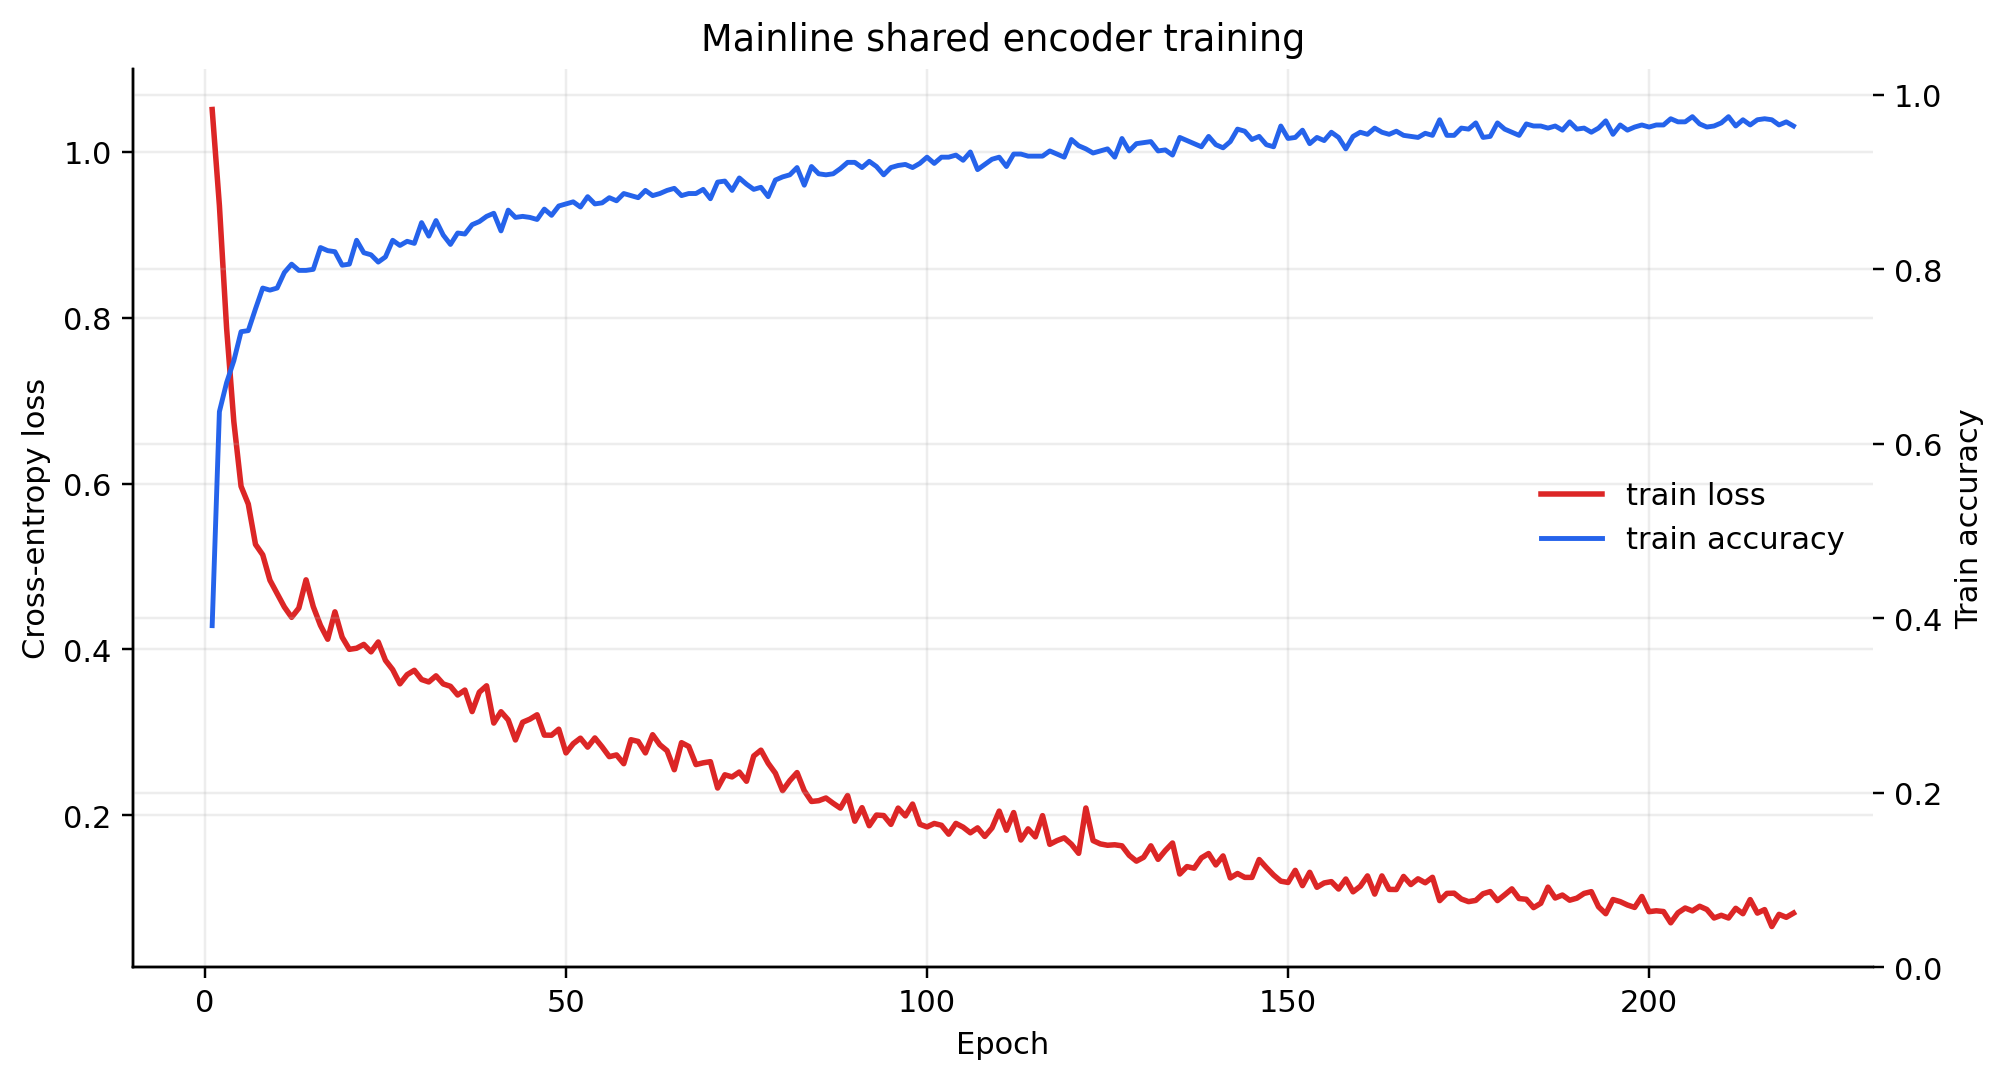
\includegraphics[width=0.88\linewidth]{competition/mainline_encoder_training.png}
\caption{主线共享小型 MLP encoder 的训练曲线。该 encoder 接收筛选后的 FBCSP 特征，并为经验库检索与候选头扫描提供 embedding。}\label{fig:mainline-training}
\end{figure}

训练共 220 个 epoch，最终交叉熵损失为 0.082，训练准确率为 96.43\%。Loss 持续下降且 accuracy 逐渐趋稳，说明小型 encoder 已充分拟合训练集；但较高训练准确率不能单独证明泛化能力，因此还要结合独立 evaluation 的 PCA、累计指标和混淆矩阵判断。该网络只生成主线使用的表示，不替代 FBCSP 主干。

\begin{figure}[H]\centering

\includegraphics[width=0.82\linewidth]{competition/mainline_embedding_pca.png}
\caption{主线 embedding 的 PCA 可视化。圆点为训练窗口，叉号为 518 个 held-out evaluation 窗口；颜色表示 left、right、foot。PCA 仅用于二维诊断，不是实际分类器。}\label{fig:mainline-embedding}
\end{figure}

PCA 图中训练与 evaluation 的同类样本总体落在相近区域，说明冻结 encoder 在回放集合上仍保留了主要类别结构。Foot 在左上区域相对集中，right 多位于下方，left 分布范围最广；left 与 right 在中部存在明显重叠，和后续混淆矩阵中的左右手误判一致。Evaluation 叉号没有完全脱离训练圆点，但类内离散和类间交叠仍较大，这解释了为什么主线需要候选特化和拒识，而不能只依赖一个固定 embedding 分类头。

\begin{figure}[H]\centering
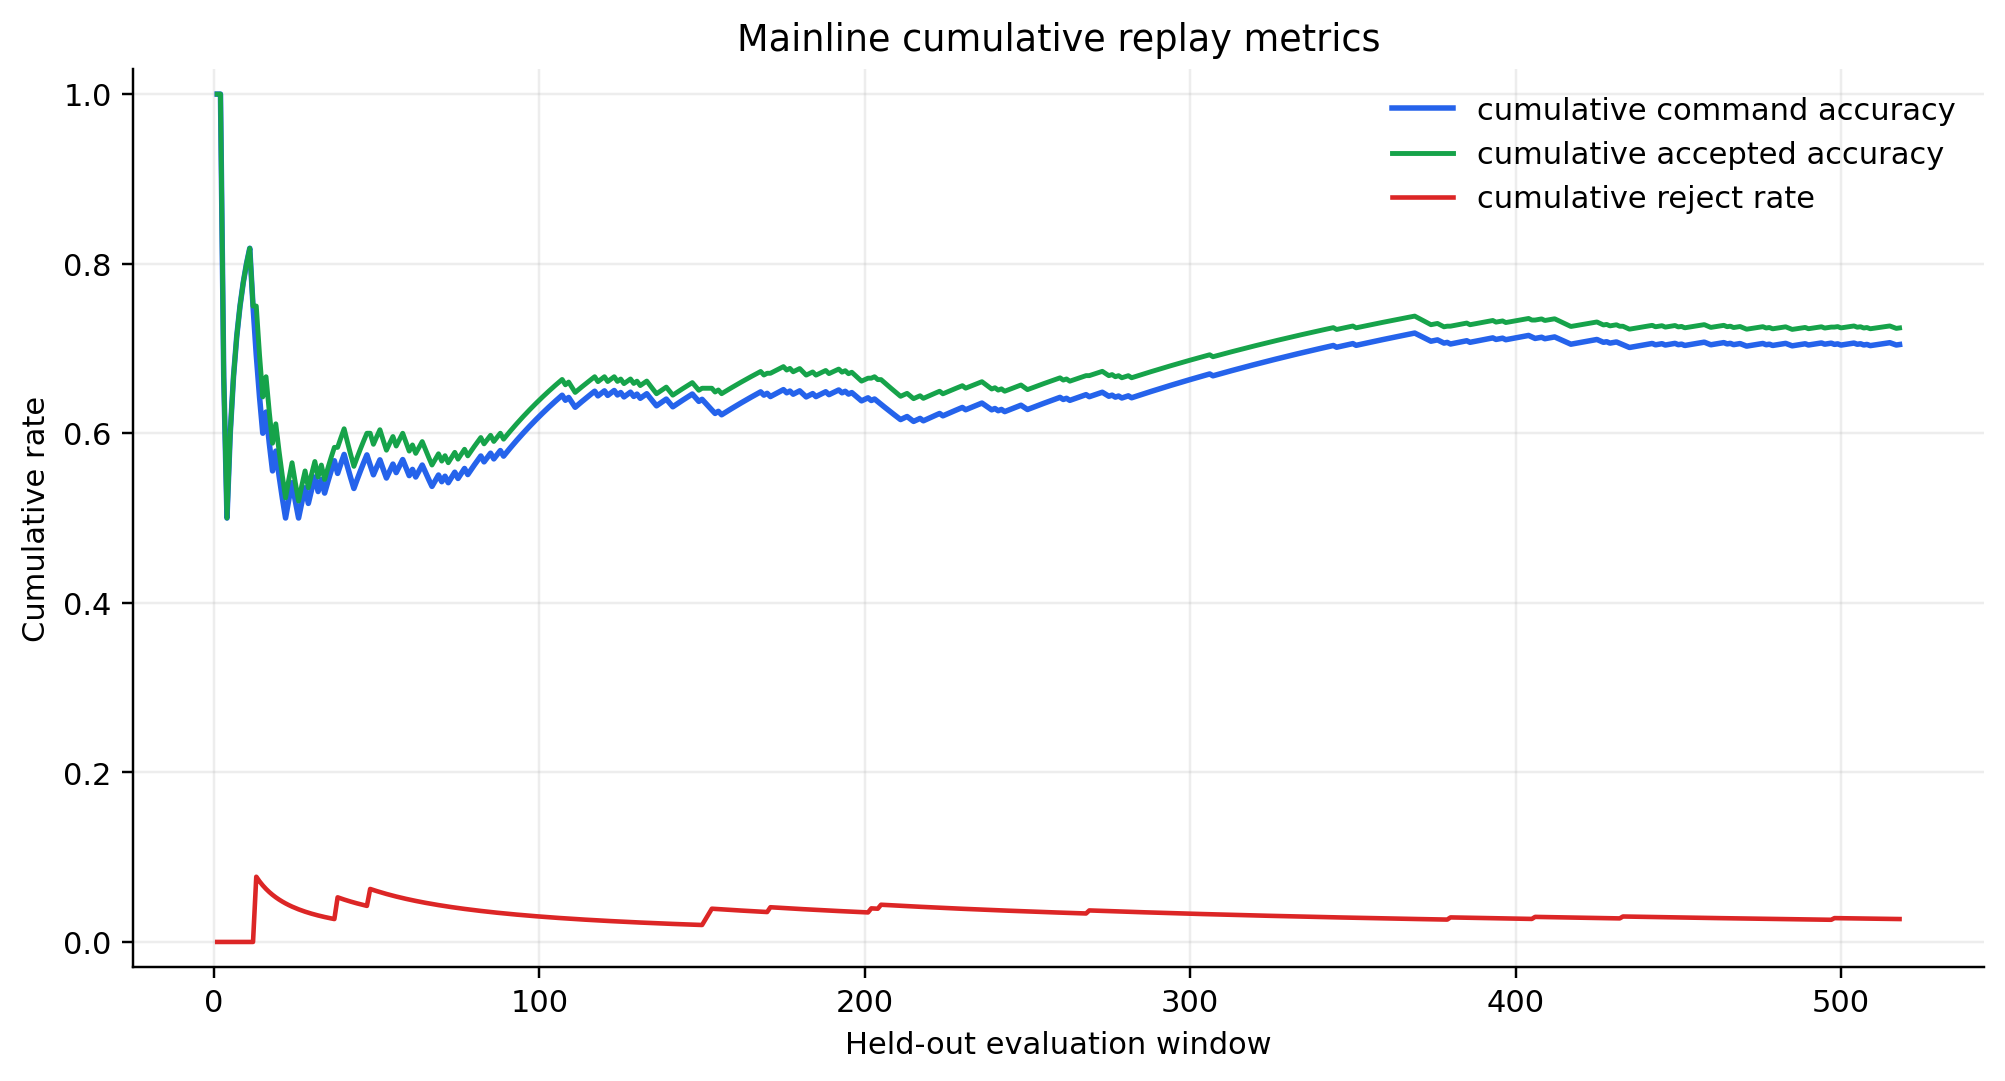
\includegraphics[width=0.88\linewidth]{competition/mainline_cumulative_metrics.png}
\caption{主线在 518 个 held-out evaluation 窗口上的累计指标。蓝线为累计指令准确率，绿线为累计接受窗口准确率，红线为累计拒识率。}\label{fig:mainline-cumulative}
\end{figure}

累计曲线在最初少量窗口中波动较大，约 300 个窗口后逐渐稳定，最终收敛到指令准确率 70.46\%、接受窗口准确率 72.42\% 和拒识率 2.70\%。绿线始终略高于蓝线，说明拒识去除了一部分不可靠窗口，但二者差距较小，当前阈值只进行了较温和的安全筛选。该图使用从第一个 evaluation 窗口开始的 cumulative 统计，与后面的固定宽度 rolling 曲线含义不同。

\begin{figure}[H]\centering
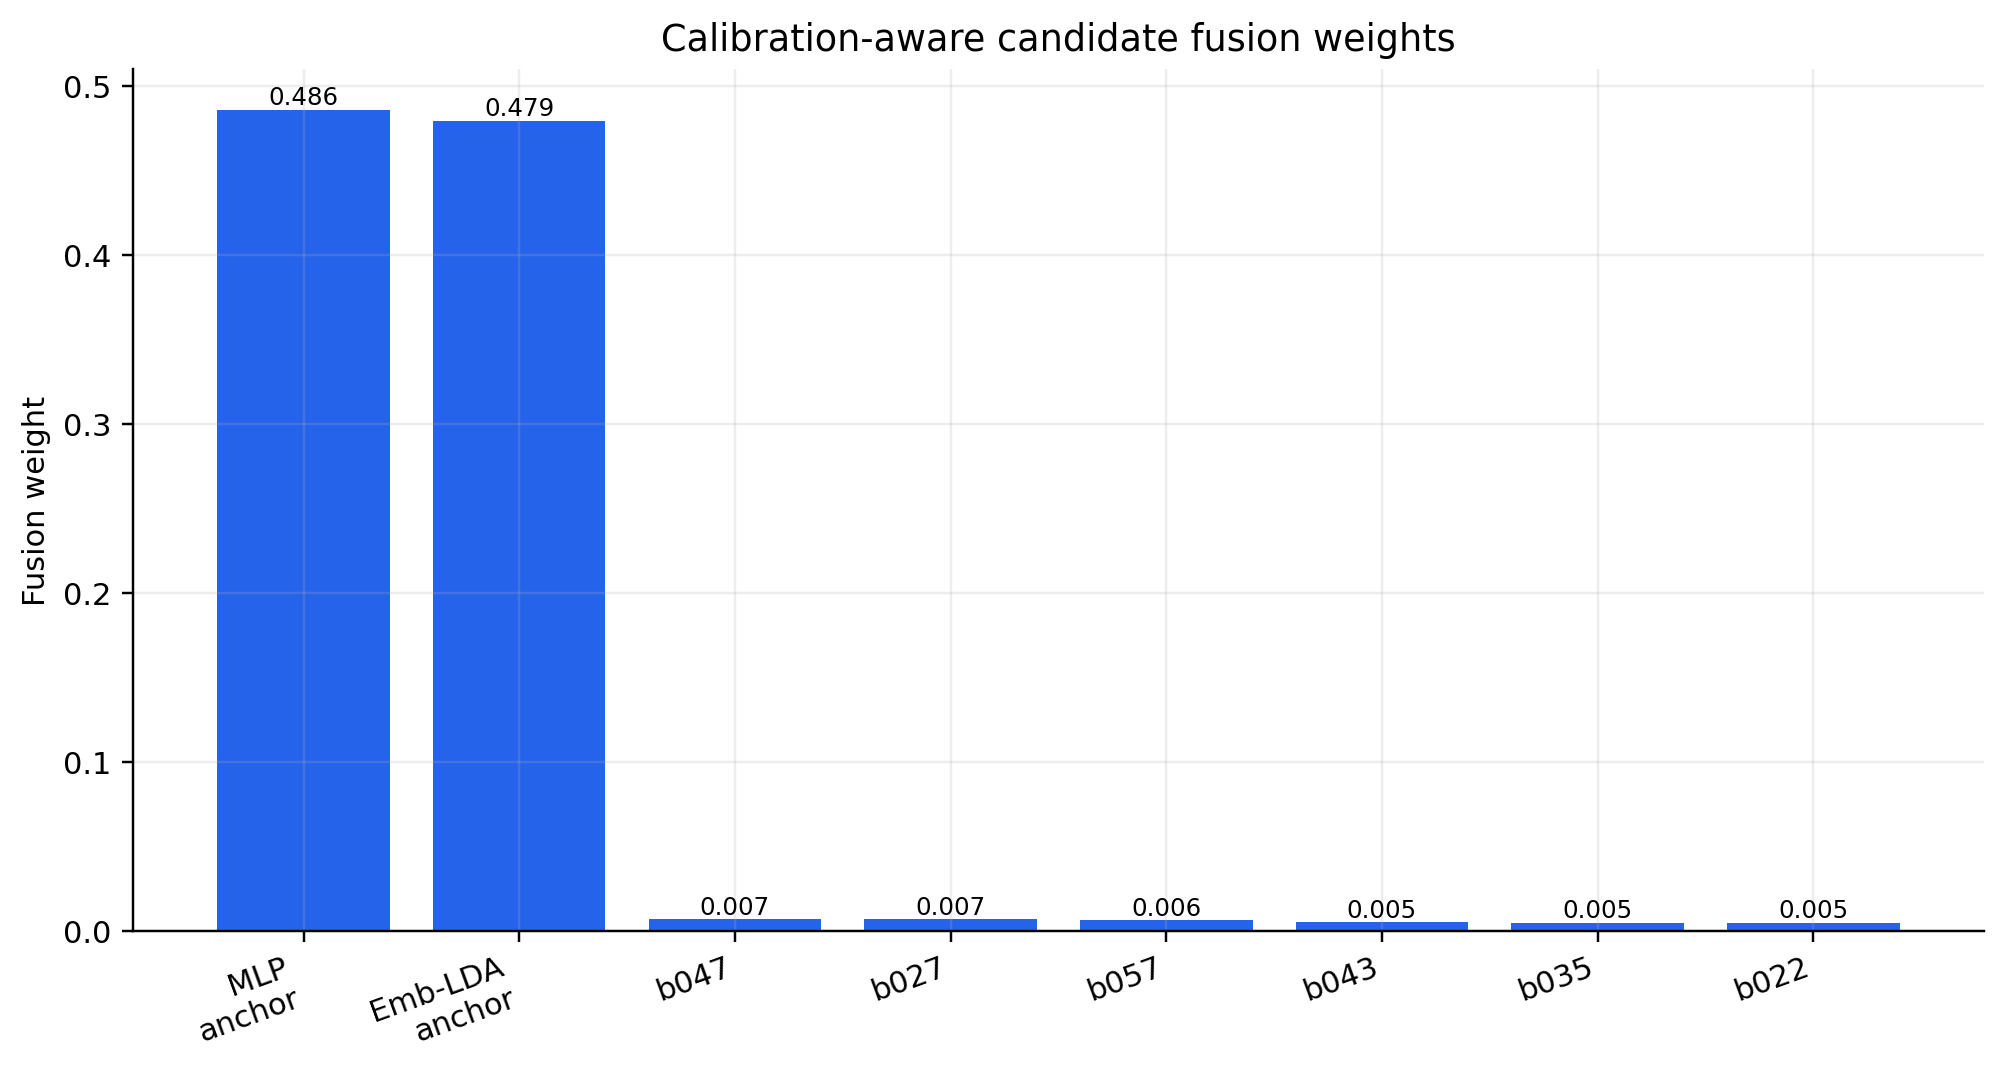
\includegraphics[width=0.88\linewidth]{competition/mainline_retrieval_weights.png}
\caption{主线经验库的候选融合权重。当前权重综合距离、训练准确率、校准准确率、校准置信度和锚点先验；两个全局锚点获得主要权重。}\label{fig:retrieval-weight}
\end{figure}
\begin{figure}[H]\centering

\includegraphics[width=0.88\linewidth]{competition/mainline_candidate_head_quality.png}
\caption{主线经验库中候选线性头的训练质量分布。红点表示参与本次扫描的候选。}\label{fig:candidate-quality}
\end{figure}
\begin{figure}[H]\centering

\includegraphics[width=0.88\linewidth]{competition/mainline_replay_traces.png}
\caption{主线候选扫描的回放轨迹。曲线分别给出滚动指令准确率与拒识率。}\label{fig:mainline-traces}
\end{figure}
\begin{figure}[H]\centering
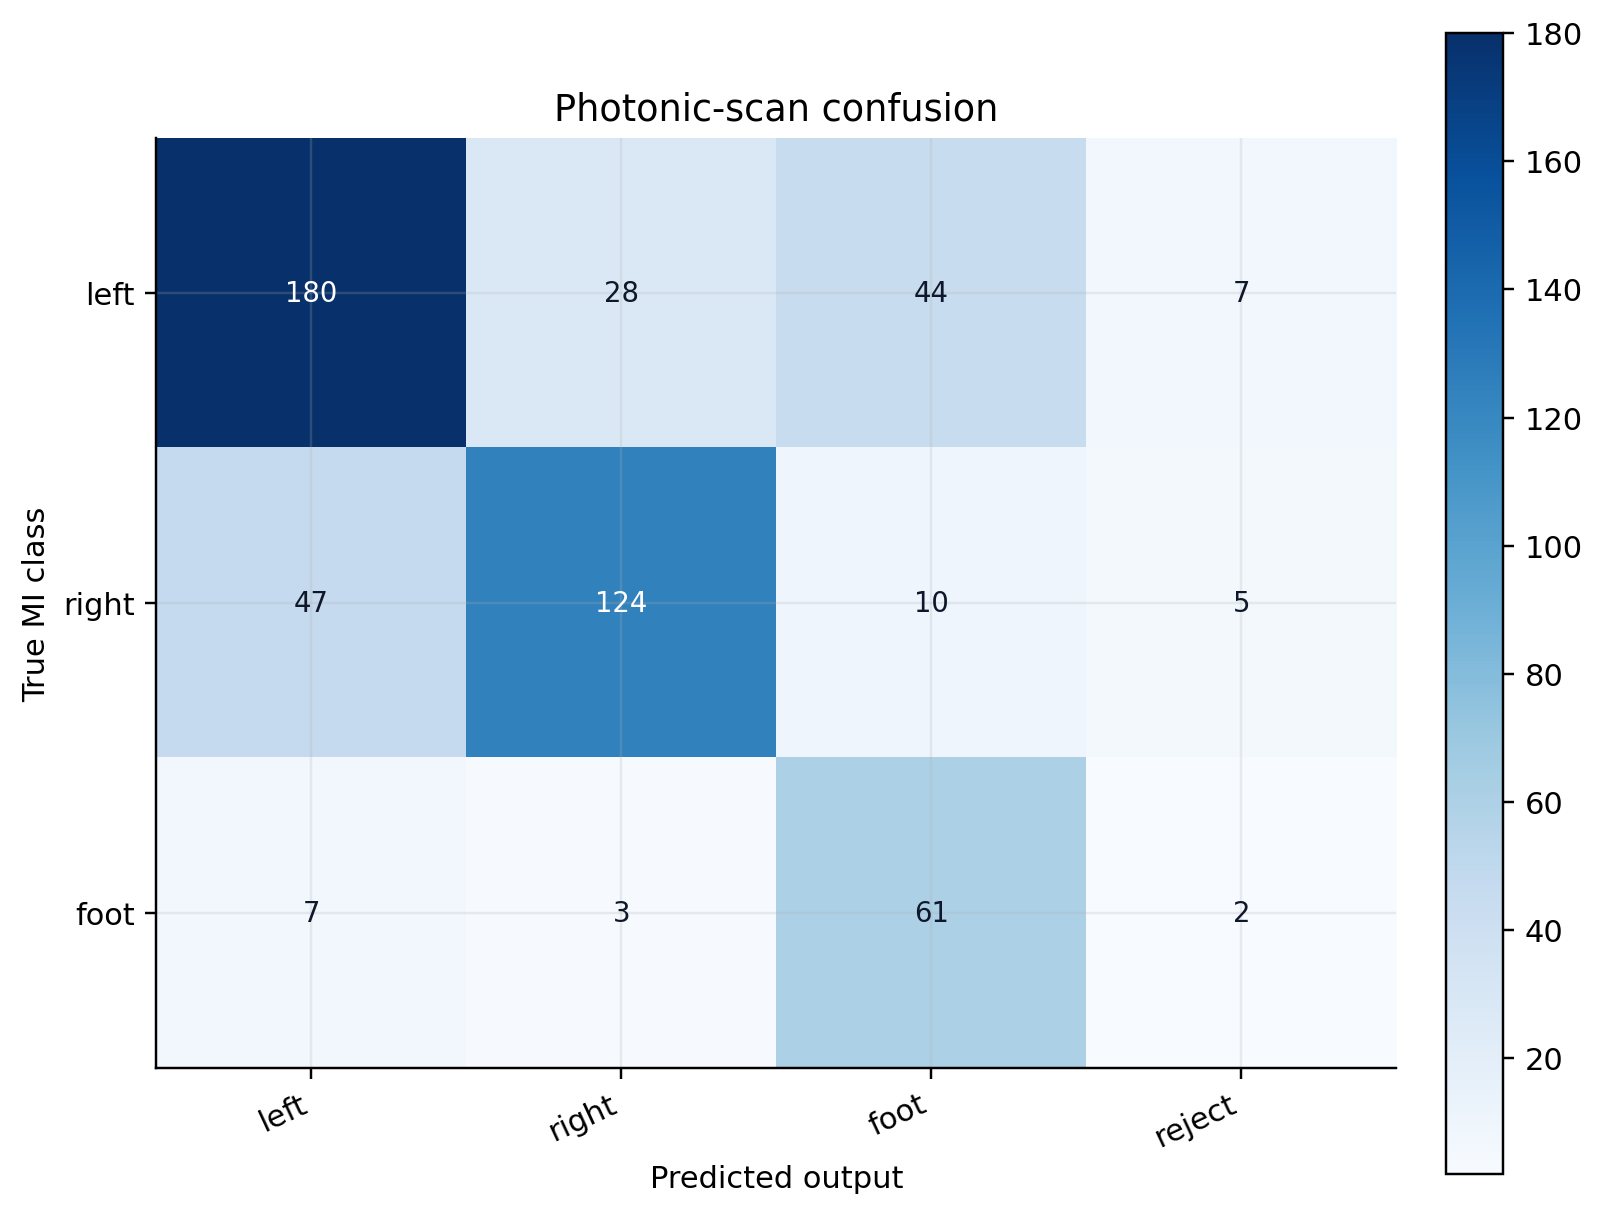
\includegraphics[width=0.76\linewidth]{competition/mainline_confusion.png}
\caption{主线候选扫描的混淆矩阵。横轴为系统输出，纵轴为真实运动想象类别。}\label{fig:mainline-confusion}
\end{figure}

混淆矩阵表明不同 MI 命令仍存在类别间混淆；reject 主要用于低置信度或小边际窗口。提高阈值通常会提高 accepted accuracy，但也会减少可输出命令数量，因此不能只追求更高拒识率。真实采集中的疲劳、注意力、眨眼和肌电还会增加低质量窗口，拒识的价值是降低错误命令，而不是简单掩盖分类失败。

\subsection{BNCI 个体特化结果}
在 BNCI2014\_004 的 9 位被试实验中，主线在 1296 个评估窗口上的平均准确率为 74.92\%，接受窗口准确率为 76.22\%，拒识率为 1.62\%。同协议下，LDA baseline 的平均准确率为 75.46\%，小型 MLP 为 74.38\%。当前主线总体平均值未超过 LDA，因此不能把经验库写成已经稳定提升精度；其已验证价值是把少量会话校准、候选模型特化和 photonic scan 连成可复现路径。后续应重点报告每位被试的收益差异，并对校准窗口数、top-$K$ 和经验库规模进行消融。

\section{运行方式与技术数据}
从工程根目录安装依赖后，完整三线对比使用
\begin{center}\small\path{python examples/run_fbcsp_design_comparison.py}\end{center}
只运行主线使用
\begin{center}\small\path{python examples/run_experience_photonic_line.py}\end{center}
单个 evaluation 窗口的完整前向使用
\begin{center}\small\path{python examples/run_single_window_inference.py --evaluation-index 0}\end{center}
其中 \texttt{evaluation-index} 是 evaluation split 内部索引，不是原始 trial 编号。BNCI 个体特化和图表重绘分别使用
\begin{center}\small
\path{python examples/run_bnci2014_004_personalization.py}\\
\path{python visualization/generate_fbcsp_design_figures.py}
\end{center}

主结果写入 \path{artifacts/metrics/fbcsp_design/summary.json}，逐算子账本写入 \path{compute_accounting.json}，运行步骤和耗时写入 \path{run_progress.json}；主线的数组、概率、rolling/cumulative 轨迹和混淆矩阵保存在 \path{experience_photonic/arrays.npz}。BNCI 目录另外保存 subject rows，便于检查个体差异。回归测试命令为
\begin{center}\small\path{python -m unittest discover -s tests}\end{center}

随附技术数据保留源码、pure runtime、examples、tests、JSON/NPZ 指标、绘图脚本、环境说明和数据下载说明。受许可证限制的大型公开数据不重复打包。提交前删除本机数据库、串口配置、缓存、绝对路径和个人信息，并检查 PDF 元数据与视频片尾。

\chapter{OpenBCI Cyton 上位机扩展}
当前 Cyton 在线采集与上位机能力\textbf{未完成}。工程中已有 acquisition adapter、控制器数据模型、SQLite 经验存储和 Tk 界面骨架，但尚未在真实被试条件下完成稳定数据采集、时序检查、质量门控、在线推理和控制反馈闭环。因此，前文准确率均来自公开数据回放，不能表述为 Cyton 在线实采准确率。

目标采集链从 BrainFlow/Cyton 数据包开始，核验采样率、样本序号和时间戳，将 ADC 计数换算为微伏并映射到 C3/C4/Cz 等电极；连续数据写入环形缓冲区，再按固定窗口长度和步长触发 pure runtime。真实联调还需补充断线恢复、坏通道处理、滤波状态连续性和长时间内存稳定性测试。

上位机计划支持少量校准引导、被试/session 元数据、经验条目新增/删除/分组、模型版本与阈值选择，以及连接状态、信号质量、预测概率、置信度和拒识原因显示。只有通过质量检查且校准/评估指标满足要求的会话才能写入经验库；低质量、过期或错误条目需要可删除和回滚。上述功能是正在开发和验证的原型目标，不作为当前已交付闭环能力。

\chapter{局限性}
当前实验主要基于公开数据集回放。公开 trial 具有固定事件边界和真值标签，不能完全代表真实在线环境中的电极漂移、无明确意图窗口、注意力变化和连续伪迹；真实在线也没有即时标签，无法直接计算实时 accuracy。两级拒识中的分类置信度拒识已有回放证据，而采集前质量门控仍需在真实数据流中验证。

当前 photonic backend 是软件量化、切片和接口路由，不是真实光芯片的逐算子执行证据。100\% forward linear share 表示全部前向线性 MAC 已按工程口径交给 backend 接管，不等于真实功耗占比、吞吐或端到端加速比。候选扫描使用单次 4-bit；其他路径采用仍在完善的自适应 4/6/8-bit 逻辑精度并拆成 4-bit 物理 slice。当前策略不是最终工程配置，现有三窗口 A/B 只构成初步误差证据，仍需在完整评估集和真实硬件上验证 slice 数、量化噪声、部分和累加误差与拒识率之间的关系。

主线在当前 BCICIV 和 BNCI 平均准确率上未稳定超过 LDA baseline，说明经验库特化仍依赖被试、校准量、top-$K$ 和条目质量。FBCSP 滤波与空间投影在在线系统中也可能构成延迟瓶颈。Cyton 上位机与真实闭环未完成，因此本文结论只能覆盖公开数据回放、光计算模拟器接口和计算账本，不能外推为真实被试部署效果。

\chapter{后续工作}
第一步是保持上层算法接口不变，接入官方模拟器和真实光芯片驱动，逐算子验证 FBCSP、标准化、MLP、候选扫描与融合的数值误差、调用次数、时延、吞吐和功耗。硬件报告需要区分软件参考、模拟器和真实芯片结果，不能继续只用 MAC 标签替代执行证据。

第二步是扩展混合精度评估。以当前 4/6/8-bit 单调升级和 8-bit shadow 机制为起点，对候选单次 4-bit、不同逻辑精度的 4-bit 位权拆分、原生更宽物理单元和可选量化感知训练进行对比；逐算子搜索满足 command accuracy、accepted accuracy 和 reject rate 的最低精度，并同时统计 slice/tile 次数、噪声鲁棒性、延迟和能耗，形成精度--效率 Pareto 选择。

第三步是完成 Cyton 上位机和真实闭环：验证连续采集、质量检查、校准、pure runtime 推理、经验库版本管理和控制反馈，建立可重复的真实被试采集协议。第四步是对经验库做校准窗口数、top-$K$、条目规模和 subject-wise 收益消融，增加条目质量评估、分组、版本、删除与回滚。最后将实验、指标、图表和报告生成进一步自动化，确保正文数字始终来自当前 artifacts。

\chapter{结论}
本文完成了一个可复现的 MI-BCI 软件原型：FBCSP 作为可解释、小样本友好的特征主干，小型 MLP 提供 embedding，经验库利用少量校准选择并加权候选线性头，低位宽 tiled MVM 完成候选扫描，数字端负责非线性、融合、质量控制和拒识。三条实验线、两套公开数据协议、指标/数组、诊断图、单窗口入口、计算账本和单元测试均已形成工程产物。

Gazelle 平台是本项目从 BCI 算法原型走向光电混合部署的关键承载平台。其基础光子矩阵计算能力与 FBCSP、标准化、小型 MLP 和候选线性头中的矩阵/向量运算具有直接接口对应关系；其中，经验库产生的多候选 head bank 能够组织为规则的 $2\times8$ tiled MVM，使个体差异驱动的候选扫描成为 Gazelle 平台最具代表性的应用路径。统一的 MatrixOpsBackend、SignalOpsBackend 和 TiledMVMBackend 又把 Gazelle 的作用从单一分类头扩展到全部前向线性计算，为算法 shape、量化策略、tile/slice 调度和硬件执行之间建立了清晰边界。

当前 Gazelle 模拟器已经接入单窗口完整前向链，并在固定 8-bit 运行中记录了 $1{,}089{,}752$ 个 bit-sliced tiles。模拟器的 476.405 s 主要来自逐 tile、逐 slice 的仿真开销，不代表评估板实机速度；按产品手册标称算力得到的 0.42 s 仅是忽略通信与调度的计算下界，不能作为实机实时性结论。仍在完善的自适应精度实验同样使用光计算模拟器；当前约 15.7\% tile 降幅等数据及其对应精度策略均待完善，不作为定版结论。Gazelle 对本项目的重要性不仅在于替换某个数字矩阵乘，更在于提供一条可量化、可调度、可验证并可进一步实机部署的光计算主干，使“EEG 特征提取--个体化经验库--多候选扫描--拒识/命令”能够形成完整的光电混合系统。

按当前 forward-only 口径，全部前向线性 MAC 已路由到 photonic backend，候选头是重点单次 4-bit、$2\times8$ tile 路径；现有证据覆盖公开数据回放、Gazelle 模拟器接口、量化调度和计算账本，真实评估板上的端到端时延、数值误差与功耗仍需进一步实测。主线已经验证“会话校准--经验库特化--候选扫描--拒识”的完整机制，但当前平均准确率未稳定超过 LDA baseline，仍需消融和真实被试验证；Cyton 上位机与真实在线闭环也尚未完成。后续工作的核心是保持现有统一接口不变，将模拟器路径迁移到 Gazelle 实机并完成真实 EEG 闭环验证。

\appendix
\chapter{线性算子与计算量清单}\label{app:ops}
表~\ref{tab:ops}按主线的一个决策窗口列出主要线性算子。这里取 $B=6$ 个频带、$C=8$ 个通道、每类 4 条 FBCSP 滤波器、$D=32$ 个特征和 $K=8$ 个候选。表中的示例使用 BCICIV\_1\_asc 的 $T=300$（marker 后 1.0--4.0 s，100 Hz）。BNCI2014\_004 的 trial 长度为 3 s、采样率为 250 Hz，应按 $T=750$ 重新计算。IIR/SOS 中的状态转移乘加按 linear MAC-equivalent 纳入，var、log、softmax 等非线性计算不放入矩阵 MAC；赛题最终是否采用相同口径，以官方定义为准。
{\small
\begin{longtable}{|L{0.17\linewidth}|L{0.22\linewidth}|L{0.16\linewidth}|L{0.13\linewidth}|L{0.13\linewidth}|}
\caption{主线前向算子、矩阵大小与计算方式}\label{tab:ops}\\ \hline
算子 & 矩阵大小/表达式 & 单窗口 MAC & 计算方式 & 当前证据 \\ \hline
\endfirsthead
\hline 算子 & 矩阵大小/表达式 & 单窗口 MAC & 计算方式 & 当前证据 \\ \hline
\endhead
CAR & $8\times T$ 通道混合 & 账本按显式线性变换统计 & SignalOps 接管 & 软件 backend \\ \hline
六频带 SOS & $B\times8\times T$ & IIR MAC-equivalent & SignalOps 接管 & 软件 backend \\ \hline
OVR CSP 投影 & $B\times3\times(4\times8)(8\times T)$ & $6\times3\times4\times8\times300=172{,}800$ & MatrixOps 接管 & bit-sliced 光计算模拟器 \\ \hline
标准化仿射 & $(32+1)\times32$ & $1{,}056$ & MatrixOps 仿射 & bit-sliced 光计算模拟器 \\ \hline
MLP 第一层 & $(64\times33)(33\times1)$ & $2{,}112$ & MatrixOps MVM & bit-sliced 光计算模拟器 \\ \hline
MLP 第二层 & $(32\times65)(65\times1)$ & $2{,}080$ & MatrixOps MVM & bit-sliced 光计算模拟器 \\ \hline
候选头扫描 & $8\times(3\times33)(33\times1)$ & $792$ & 80 个 $2\times8$ tile & 单次 4-bit 光计算模拟器 \\ \hline
候选概率融合 & $(1\times8)(8\times3)$ & $24$ & MatrixOps 线性组合 & 软件 backend \\ \hline
\end{longtable}
}
表中的“接管”表示算子已进入统一软件 backend 和计算账本，不表示已经在真实光芯片上执行。候选头是当前低位宽路径中最适合批量处理的线性计算；式~\eqref{eq:scan} 已按 tile 切分。后续替换执行核时，必须逐项补充实际调用、读回误差、slice/tile 数、时延和功耗，不能只保留理论 MAC。

\chapter{提交材料核查表}
\begin{table}[H]\centering
\caption{与赛题技术文档要求的对应关系}\label{tab:checklist}
\begin{tabularx}{0.95\linewidth}{|p{0.29\linewidth}|X|}\hline
要求 & 本文/技术数据位置 \\ \hline
核心内容快速预览 & 封面后第 1 页，目录前 \\ \hline
功能、架构、算法、设计与结果 & 第 1--4 章及图\ref{fig:system}、图\ref{fig:fbcsp-flow}、图\ref{fig:photonic-mapping}和图\ref{fig:mainline-confusion} \\ \hline
线性层矩阵大小、计算量和光计算标记 & 第 3 章与附录 A；backend 接管、光计算模拟器和硬件未实测边界明确 \\ \hline
注释源码、测试数据、设计一致 & 工程源码根目录、tests 测试目录、artifacts/metrics 指标目录与第 4 章 \\ \hline
PPT 和演示视频支撑 & 系统图、结果图和公开数据回放；不得把 Cyton/真实硬件写成已完成 \\ \hline
匿名与敏感信息控制 & 无可识别机构、人员或标识；提交前再次检索文件名、PDF 元数据和视频片尾 \\ \hline
\end{tabularx}
\end{table}

\printbibliography[heading=bibintoc,title={参考文献}]
\end{document}
